\documentclass[12pt]{article}
\usepackage[margin=1in]{geometry}
\usepackage{booktabs}
\usepackage{float}
\usepackage{amsmath}
\usepackage{graphicx}
\usepackage{hyperref}
\usepackage{setspace}
\usepackage{longtable}
\usepackage{array}
\usepackage{enumitem}
\onehalfspacing

\title{Kazakhstan--China Economic Diplomacy and Structural Trade Asymmetry:\\
A Theoretically Integrated Journal-Length Analysis, 2015--2024}
\author{}
\date{April 2026}

\begin{document}
\maketitle

\begin{abstract}
This paper develops a theory-led and empirically grounded account of Kazakhstan--China economic diplomacy under conditions of asymmetric interdependence. Using only existing project outputs for 2015--2024, it integrates geoeconomics, Belt and Road Initiative (BRI) scholarship, multivector foreign policy theory, and small-state agency debates into a unified analytical framework. The empirical core documents a late-period structural break: Kazakhstan's bilateral trade relationship with China shifts from sustained surpluses to deficits in 2023--2024, while sectoral composition remains asymmetric (commodity-heavy exports versus manufacturing-heavy imports). The paper argues that this shift does not invalidate multivectorism as a doctrine, but it raises the policy threshold for maintaining strategic autonomy. Methodologically, the study combines descriptive structural analysis with interpretable trade indices and process-based qualitative interpretation of institutional mechanisms. The contribution is threefold: periodization of the 2015--2024 arc, integration of theory with sectoral structure, and clarification of the difference between absolute dependence and comparative dependence across partners.
\end{abstract}

\section{Introduction}
\subsection{Background and Problem}
Kazakhstan's economic relationship with China has evolved from a relatively narrow energy-centered channel into a broader system that includes manufacturing imports, logistics integration, corridor politics, and policy coordination under BRI-era institutions. This transformation unfolded in parallel with structural shocks in Eurasia, including the mid-2010s commodity cycle, pandemic-era disruption, and the post-2022 reconfiguration of regional trade routes. The central analytical question is not whether trade grew, but whether the pattern of growth became structurally asymmetric in ways that constrain Kazakhstan's policy room.

The long-standing policy narrative in Kazakhstan emphasizes multivectorism: active balancing among major external partners (China, Russia, EU, and others) to preserve sovereignty and negotiation leverage. Yet a multivector doctrine can remain formally intact while the underlying economic structure narrows in critical sectors. If dependence rises in high-substitution-cost import categories while export composition remains resource-concentrated, bargaining flexibility may erode even without formal alliance shifts.

\subsection{Research Objective}
This paper answers four linked questions:
\begin{enumerate}[leftmargin=*]
\item How did China's relative position change in Kazakhstan's trade structure compared with Russia and the EU?
\item Did bilateral trade with China become more compositionally asymmetric over 2015--2024?
\item Does the post-2022 period represent cyclical variation or structural break in the bilateral balance?
\item What do these trends imply for multivector foreign policy and small-state agency under geoeconomic pressure?
\end{enumerate}

\subsection{Contribution}
The paper contributes by converting existing project outputs into a coherent journal-style manuscript with explicit theoretical architecture. It adds depth in three ways: (1) theory integration (geoeconomics, asymmetrical interdependence, multivectorism); (2) transparent metric definitions; and (3) structured interpretation of balance, concentration, and sectoral penetration trends.

\section{Theoretical and Literature Framework}
\subsection{Geoeconomics and Statecraft}
The geoeconomics tradition frames international competition as the strategic use of economic instruments for political effect. In classical formulation, interstate influence is increasingly exercised through market access, capital allocation, supply chain integration, and infrastructure positioning. For Central Asia, this perspective is particularly relevant because transport corridors, energy routes, and industrial sourcing structures can alter bargaining power without direct military confrontation.

Applied to Kazakhstan--China relations, geoeconomics highlights two mechanisms. First, infrastructure and logistics integration can reduce transaction costs while increasing path dependence. Second, asymmetries in market scale and product complexity can produce durable leverage effects: the smaller state may find diversification more expensive than the larger state finds substitution.

\subsection{BRI, Corridor Politics, and Structural Integration}
BRI scholarship has moved from headline-level project mapping toward analyses of implementation, regional adaptation, and distributional effects. Kazakhstan's role is structurally central in overland Eurasian connectivity. Existing studies emphasize both opportunity and risk: opportunity through transit rents, investment, and market access; risk through concentration in externally controlled financing, procurement chains, and standards ecosystems.

For this paper, the BRI debate is operationalized not through project counts but through trade structure outcomes. The question is whether deepening connectivity translated into diversified export upgrading for Kazakhstan, or primarily into faster import penetration in manufactures.

\subsection{Multivectorism, Co-Alignment, and Policy Autonomy}
Multivector foreign policy is often interpreted as diplomatic balancing across major powers. A stricter political-economy interpretation treats multivectorism as the maintenance of credible alternatives across sectors. Under this interpretation, autonomy depends on preserving substitutability in strategically important economic channels.

If high-concentration sectors become locked into one partner, multivector diplomacy can survive rhetorically but weaken operationally. The concept of co-alignment is useful here: simultaneous cooperation with different powers on different issue-areas. Empirically, co-alignment requires sectoral spread rather than aggregate neutrality.

\subsection{Asymmetrical Interdependence and Small-State Agency}
Interdependence is rarely symmetric. The partner with more alternatives usually bears lower adjustment costs and thus has stronger bargaining position. This does not eliminate small-state agency; it changes the domain where agency is effective. Agency is strongest in institution design, timing, issue-linkage, and partner diversification. It is weakest when domestic capability and supplier options are both narrow.

Theoretical expectation for Kazakhstan is therefore conditional: agency should be visible where policy can influence sequencing and market access, but structural asymmetry should persist where production complexity and technological depth remain externally sourced.

\subsection{Domestic Political Economy and Societal Constraints}
A recurring finding in the broader literature is the gap between elite-level cooperation and societal skepticism toward concentrated external influence. This matters analytically because domestic legitimacy can constrain project implementation, especially in land, labor, and visible infrastructure sectors. For economic diplomacy, domestic reception is not peripheral; it conditions feasibility of long-horizon agreements.

\subsection{Gaps Addressed by This Study}
This paper addresses five gaps often left separated in prior work:
\begin{enumerate}[leftmargin=*]
\item Decade-level periodization with explicit post-2022 structural interpretation.
\item Integration of comparative partner framing (China vs Russia vs EU) with bilateral trade anatomy.
\item Joint treatment of balance shift and composition shift.
\item Direct linkage between theory claims and measurable trade indicators.
\item Clear distinction between rhetorical multivectorism and sectoral substitutability.
\end{enumerate}

\section{Methodology and Analytical Design}
\subsection{Data Scope and Constraints}
The analysis uses only existing repository outputs generated from WTO-oriented bilateral datasets and project processing scripts. The operative annual window for synthesis is 2015--2024. The paper does not introduce new series, new downloads, or new figures.

\subsection{Mixed-Method Logic}
The design combines quantitative structural description and qualitative mechanism interpretation:
\begin{itemize}
\item Quantitative component documents direction, magnitude, and composition of trade shifts.
\item Qualitative component maps those shifts onto policy mechanisms and theoretical expectations.
\end{itemize}

This is appropriate for an international political economy argument where inference depends on pattern consistency across indicators rather than on large-N causal identification.

\subsection{Core Trade Metrics}
To make the argument explicit and replicable, the paper uses interpretable index definitions.

\textbf{(1) Import Dependence on China}
\[
ID_t^{KZ\leftarrow CHN}=\frac{M_t^{KZ,CHN}}{M_t^{KZ,World}}
\]

\textbf{(2) Export Dependence on China}
\[
ED_t^{KZ\rightarrow CHN}=\frac{X_t^{KZ,CHN}}{X_t^{KZ,World}}
\]

\textbf{(3) Bilateral Asymmetry Ratio}
\[
AR_t=\frac{M_t^{KZ,CHN}}{X_t^{KZ,CHN}}
\]
where $AR_t>1$ indicates import-led asymmetry for Kazakhstan.

\textbf{(4) Revealed Comparative Advantage (Balassa-type, by sector $k$)}
\[
RCA_{k,t}^{KZ}=\frac{\left(X_{k,t}^{KZ}/X_t^{KZ}\right)}{\left(X_{k,t}^{World}/X_t^{World}\right)}
\]

\textbf{(5) Trade Intensity Index (partner orientation)}
\[
TII_t^{KZ,CHN}=\frac{\left(X_t^{KZ,CHN}/X_t^{KZ,World}\right)}{\left(M_t^{World,CHN}/M_t^{World,World}\right)}
\]

\textbf{(6) Trade Complementarity Index (sector-share compatibility)}
\[
TCI_{KZ,CHN,t}=100\left(1-\frac{1}{2}\sum_k\left|m_{k,t}^{CHN}-x_{k,t}^{KZ}\right|\right)
\]

Not all indices are estimated as full econometric models in this draft; they are used as conceptual and descriptive scaffolding consistent with available project outputs.

\subsection{Interpretive Strategy}
The interpretation proceeds in sequence:
\begin{enumerate}[leftmargin=*]
\item Establish aggregate trend and break timing.
\item Decompose by sector to identify where asymmetry is produced.
\item Compare partner channels to avoid bilateral overreading.
\item Map patterns to theory claims about dependence and agency.
\end{enumerate}

\section{Empirical Results I: Kazakhstan's External Trade Structure (Context)}
\subsection{Multipolar Structure and Reweighting}
Within the China--Russia--EU comparison set used in existing project outputs, Kazakhstan's trade profile begins the period with clear EU primacy, substantial Russia linkage, and a smaller but growing China channel. Over time, China rises while EU share declines, producing reweighting rather than pure replacement.

\begin{figure}[H]
\centering
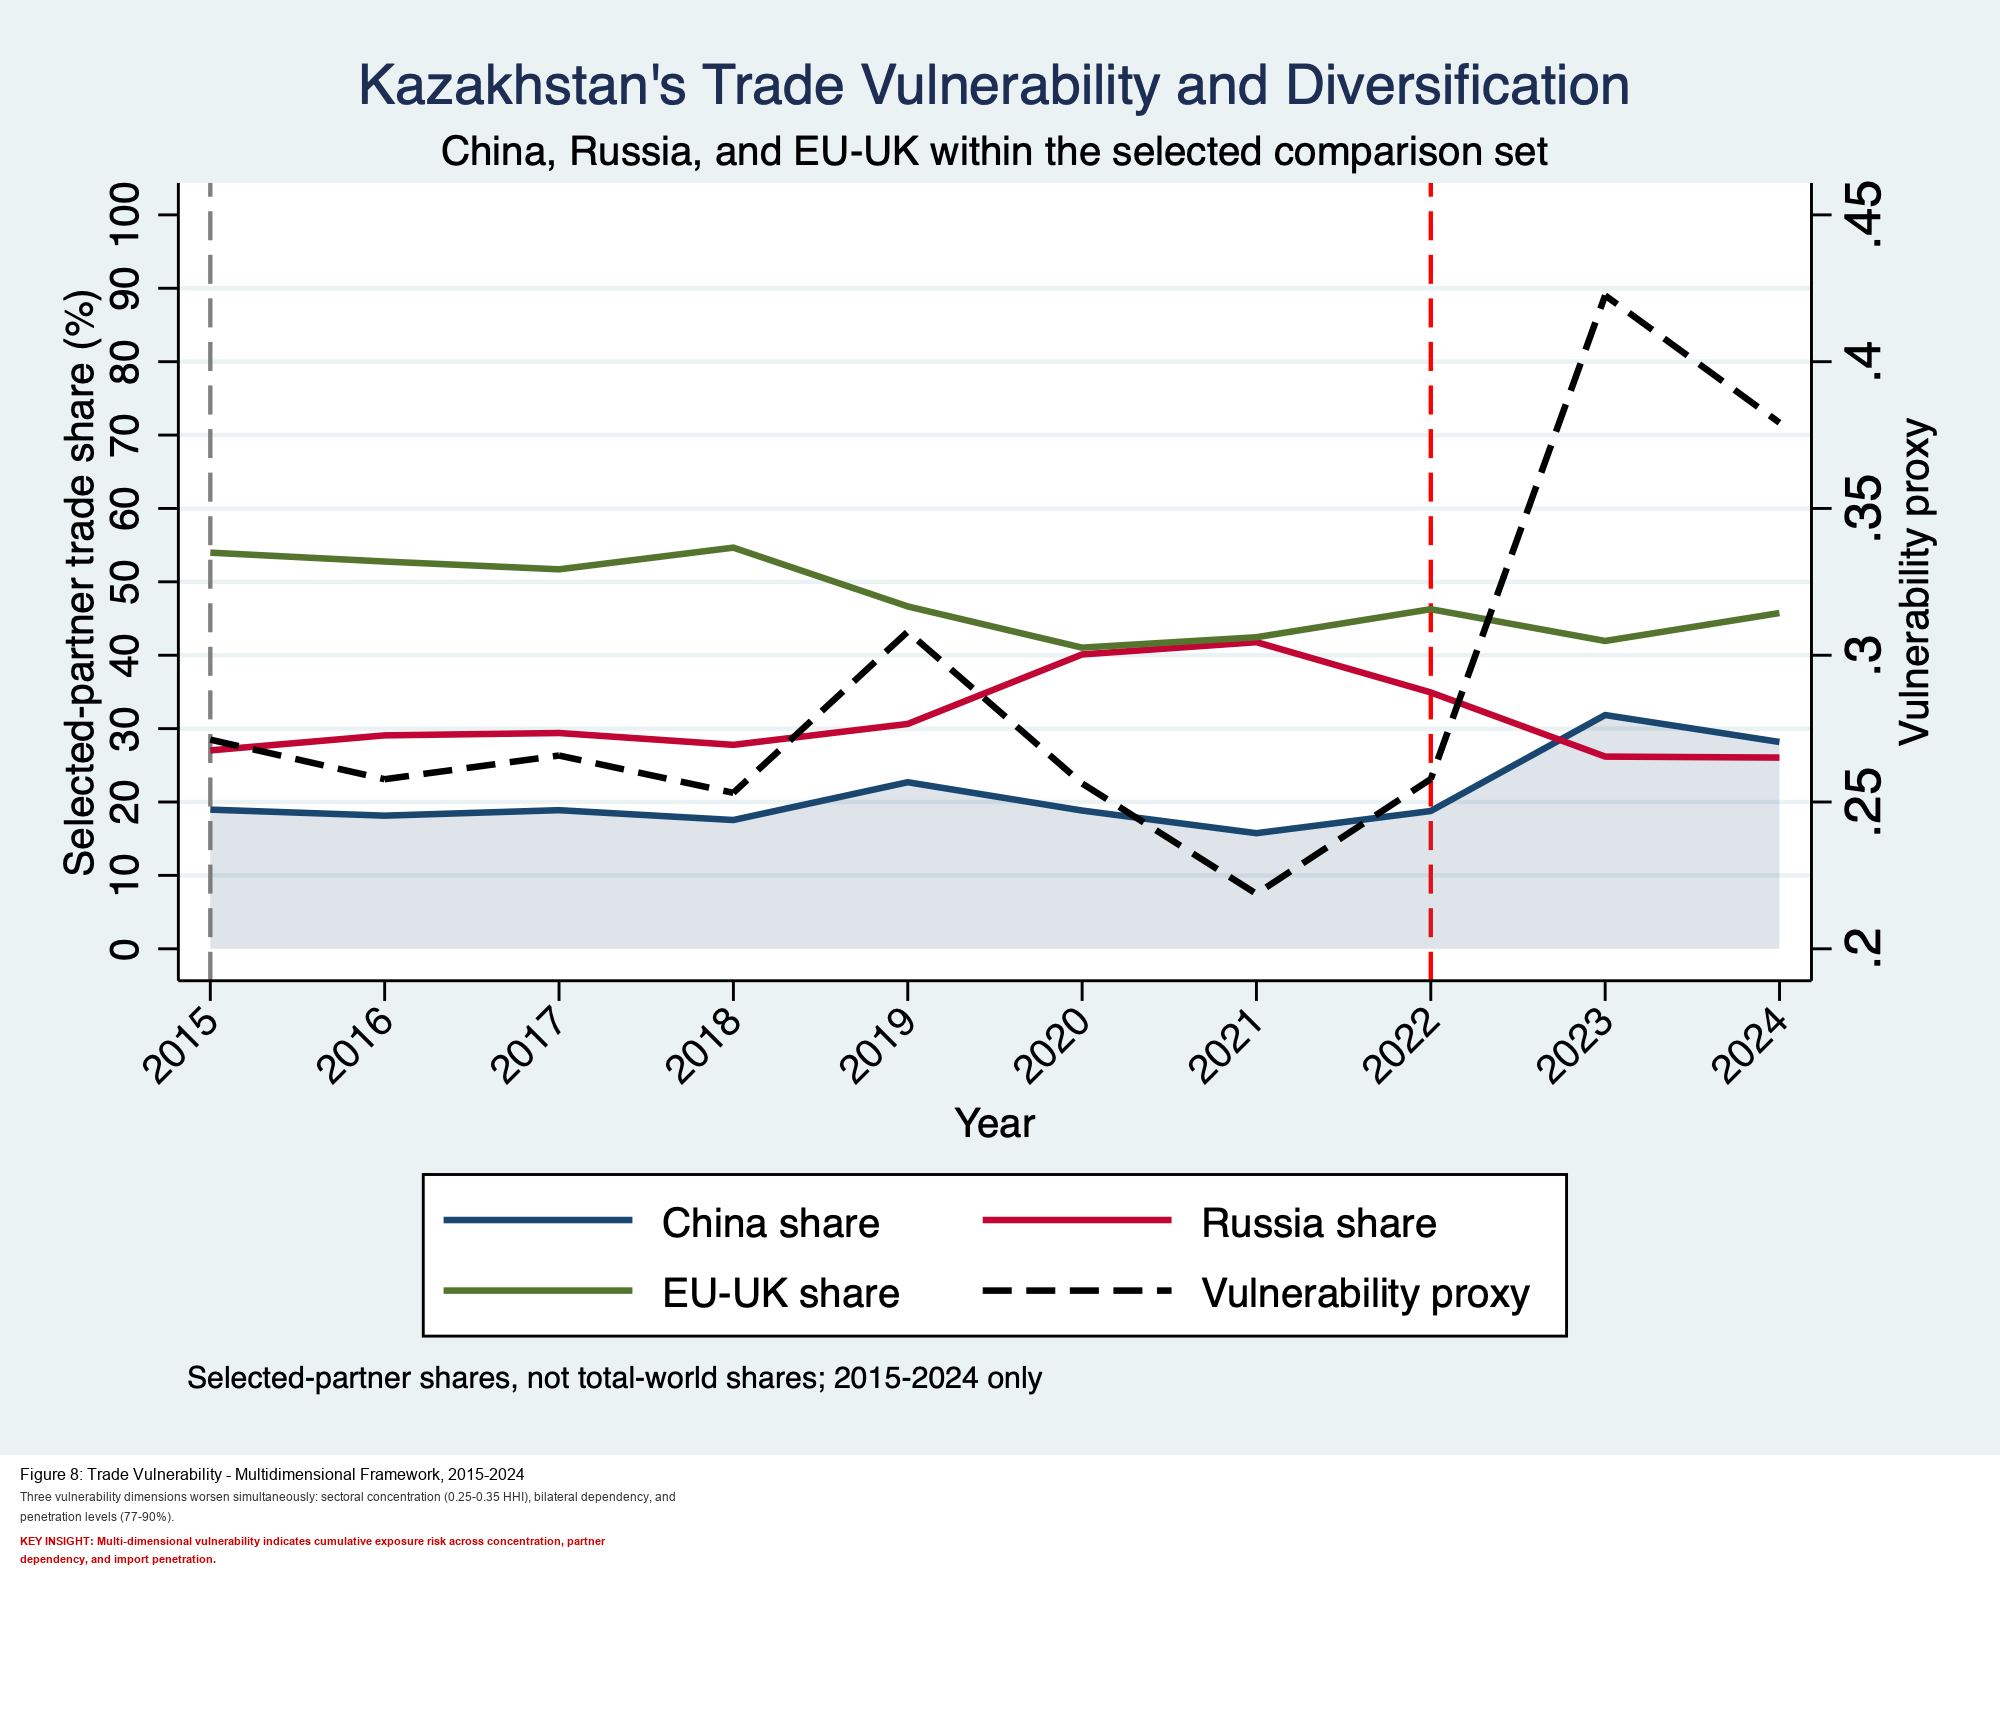
\includegraphics[width=0.94\textwidth]{figures/fig8_vulnerability_multivector_annotated.png}
\caption{Multivector partner-share dynamics from existing project outputs.}
\label{fig:multivector}
\end{figure}

\subsection{Post-2022 Shift in Relative Orientation}
The late-period acceleration is visible in partner-orientation figures. The China--Russia comparison indicates that Kazakhstan's trade structure crosses into a new relative regime after 2022, consistent with rerouting, sanctions-era market adjustments, and stronger China-linked import pull.

\begin{figure}[H]
\centering
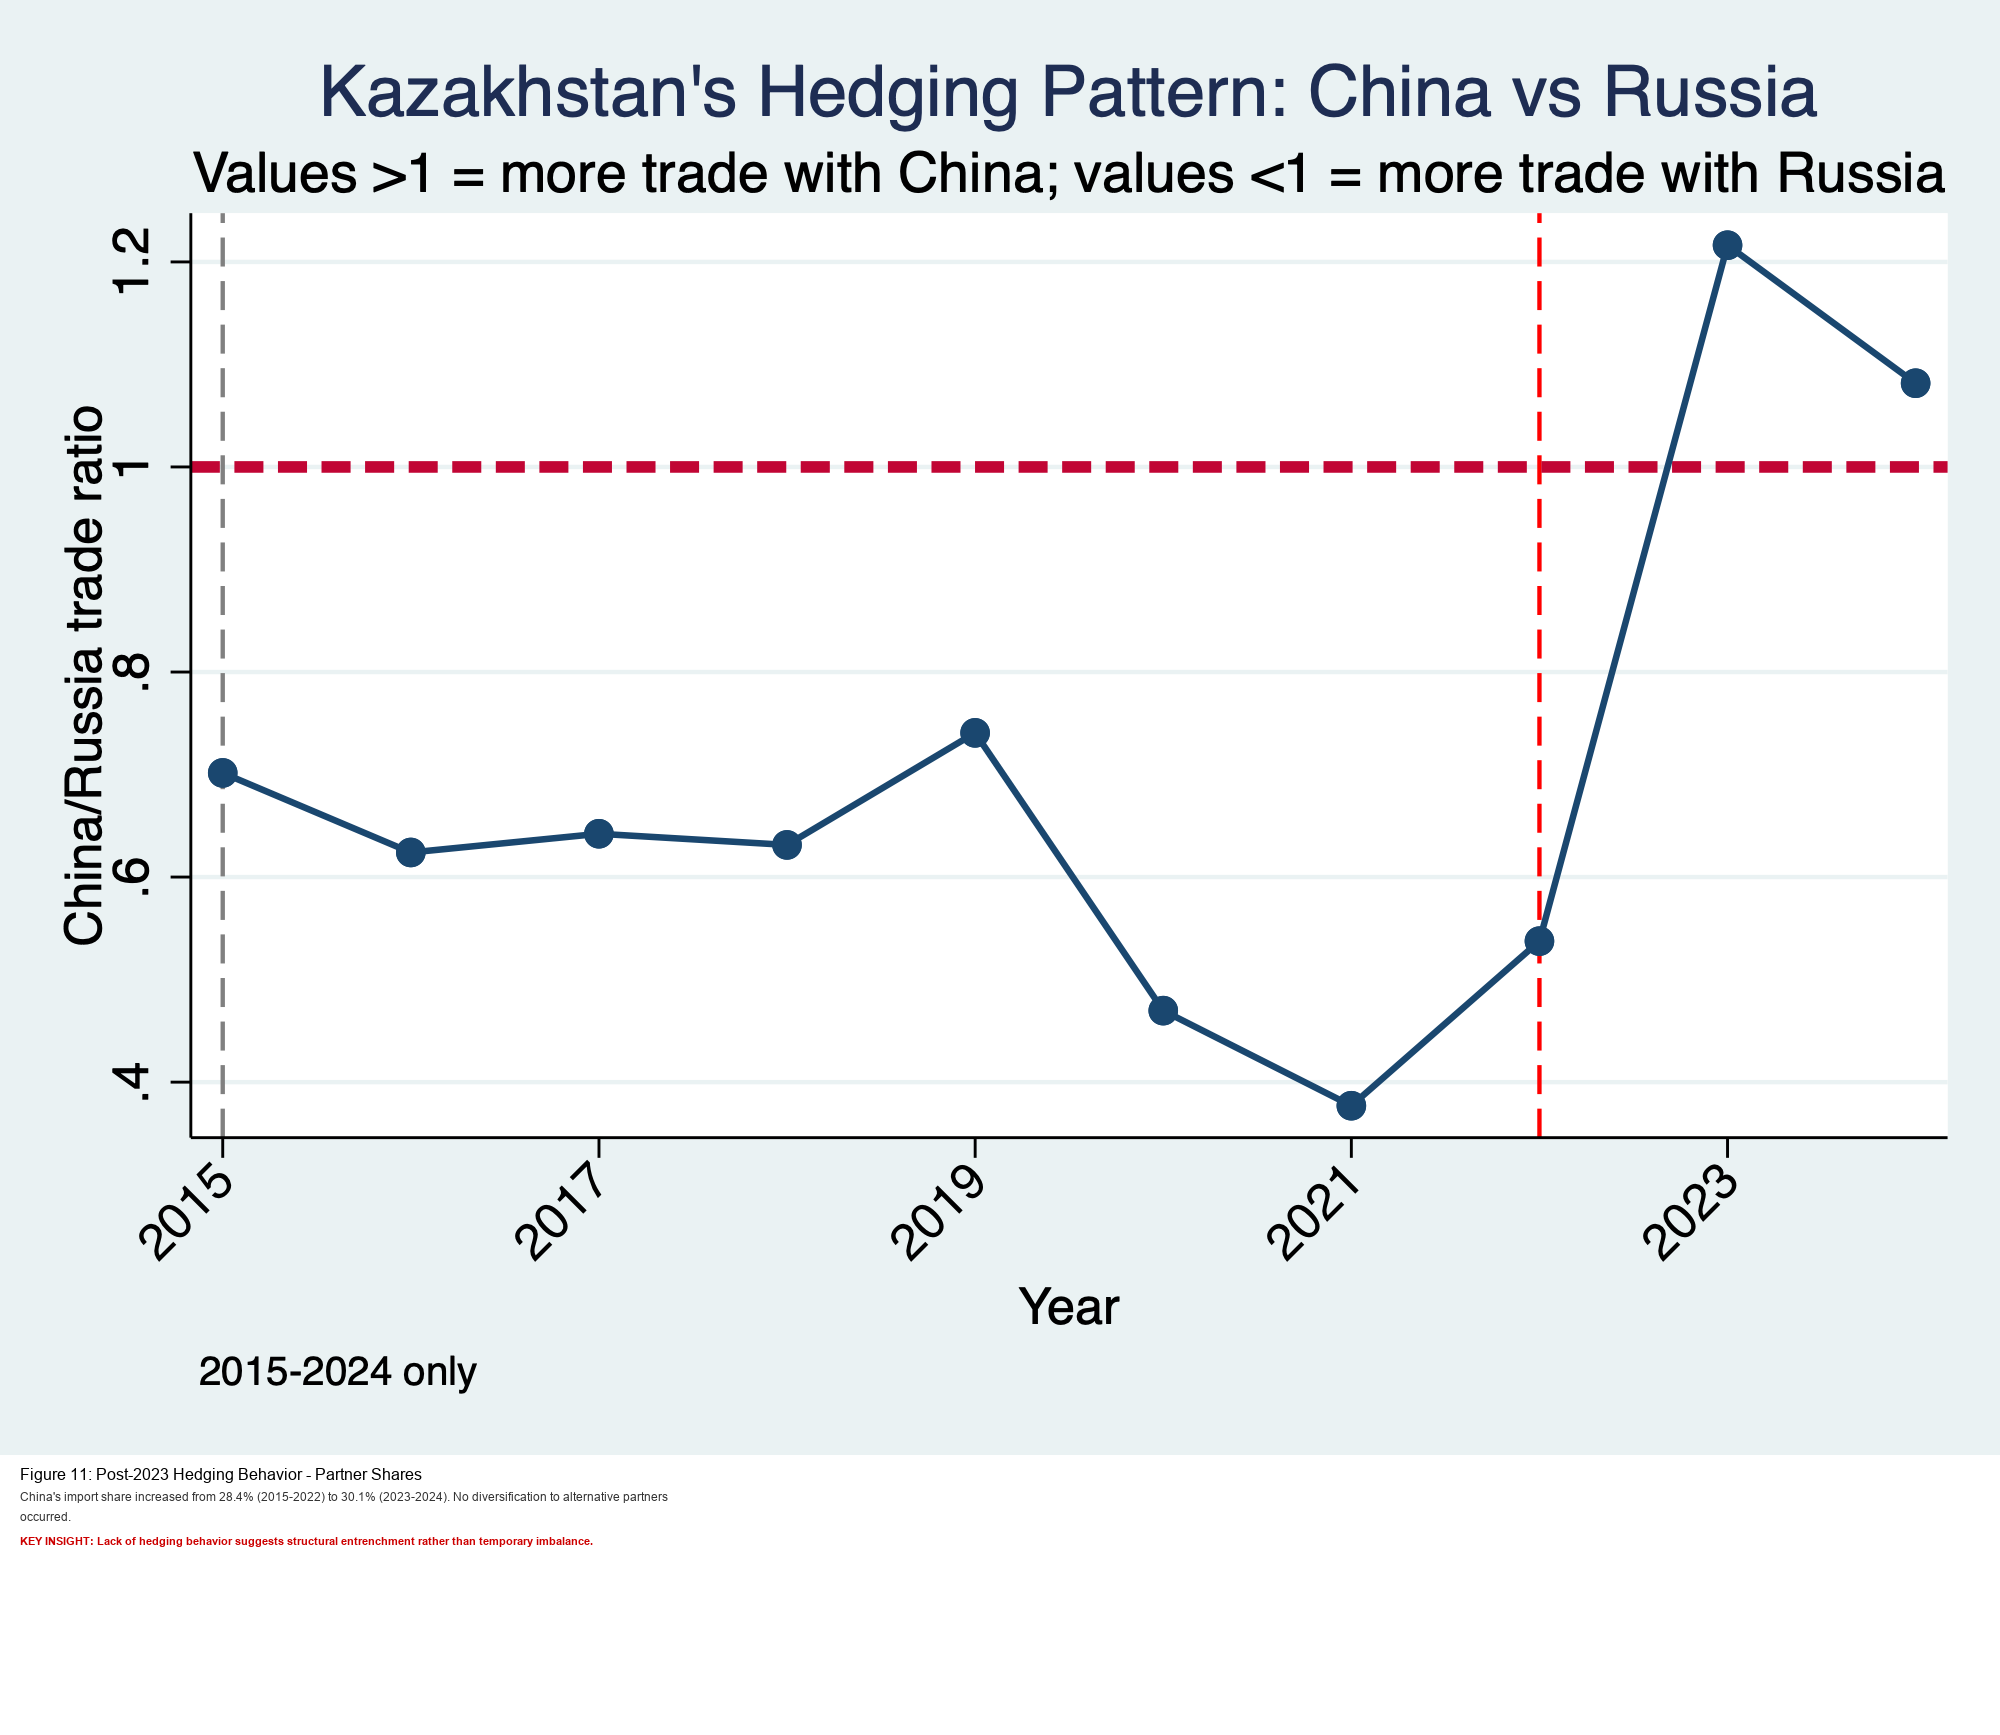
\includegraphics[width=0.94\textwidth]{figures/fig11_hedging_behavior_annotated.png}
\caption{China--Russia orientation ratio and hedging pattern (existing figure).}
\label{fig:hedging}
\end{figure}

\subsection{Interpretation}
This shift should be interpreted as structural adaptation under constraint, not linear drift. Kazakhstan remains connected to all major channels, but composition of marginal change favors China in key traded manufactures.

\section{Empirical Results II: Structural Features of Sino--Kazakh Trade}
\subsection{Scale Growth and Break Timing}
Annual bilateral totals show strong growth over the period and a clear regime break in 2023. Existing series indicate that higher total turnover coexists with balance deterioration from Kazakhstan's perspective.

\begin{figure}[H]
\centering
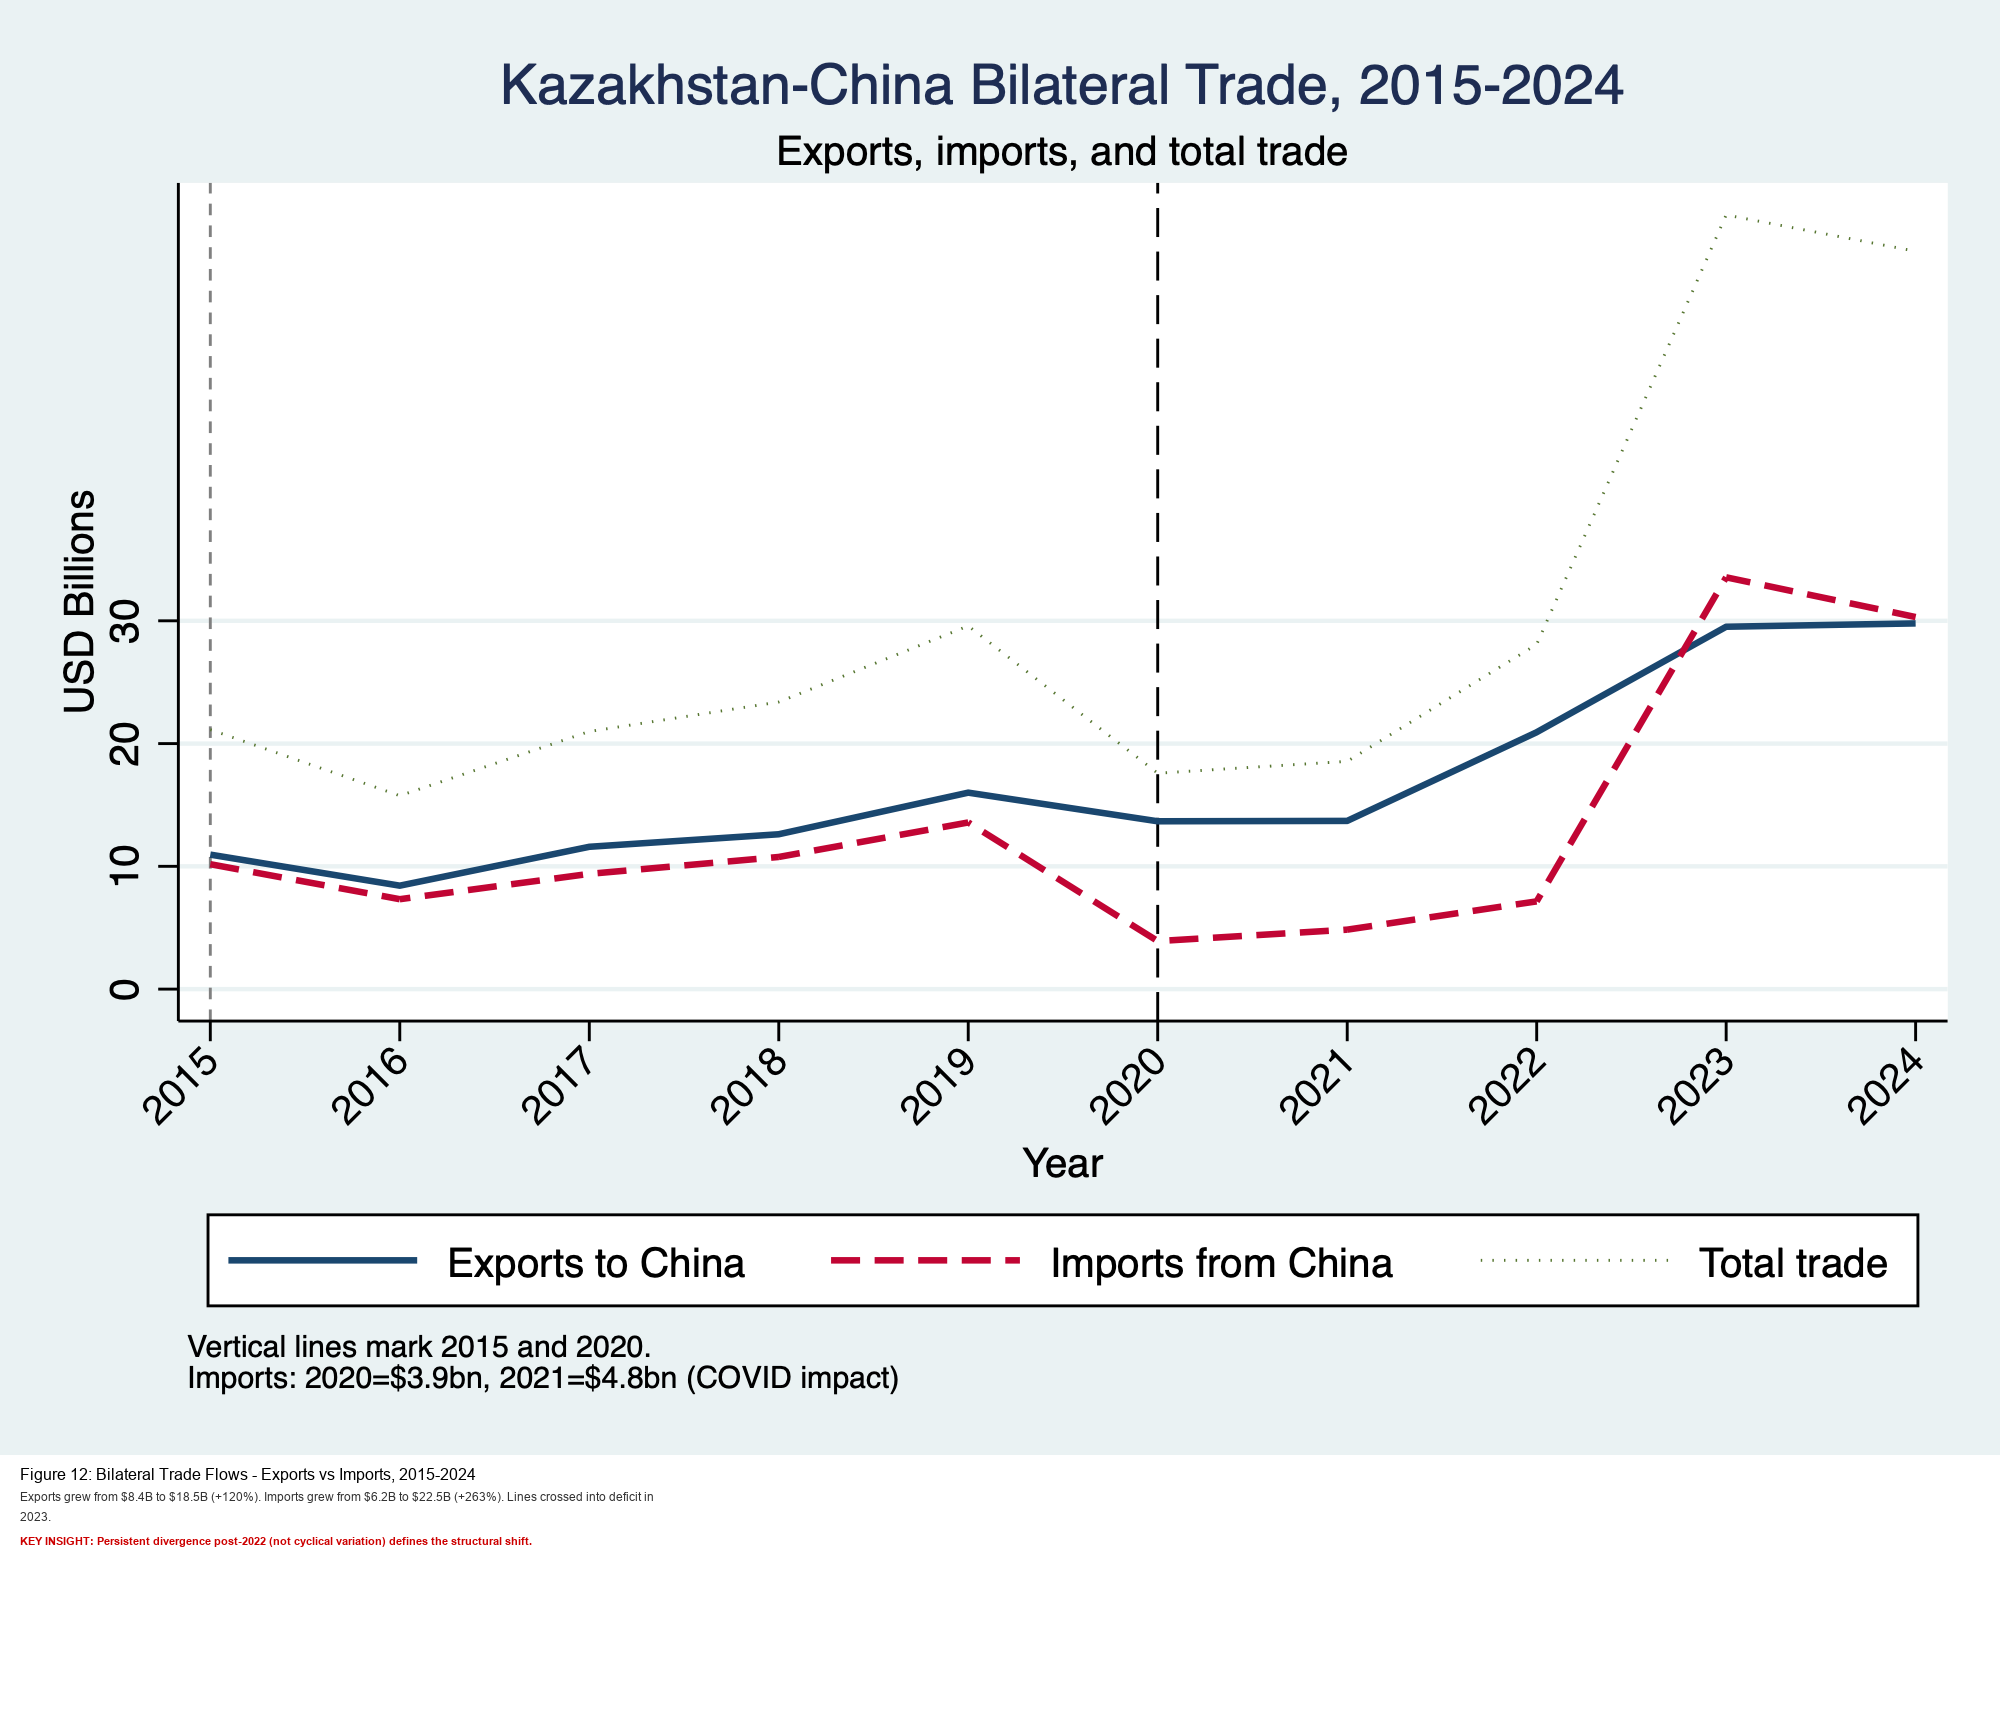
\includegraphics[width=0.94\textwidth]{figures/fig12_trade_flows_annotated.png}
\caption{Aggregate Kazakhstan--China trade flows, 2015--2024 (existing figure).}
\label{fig:flows}
\end{figure}

\begin{figure}[H]
\centering
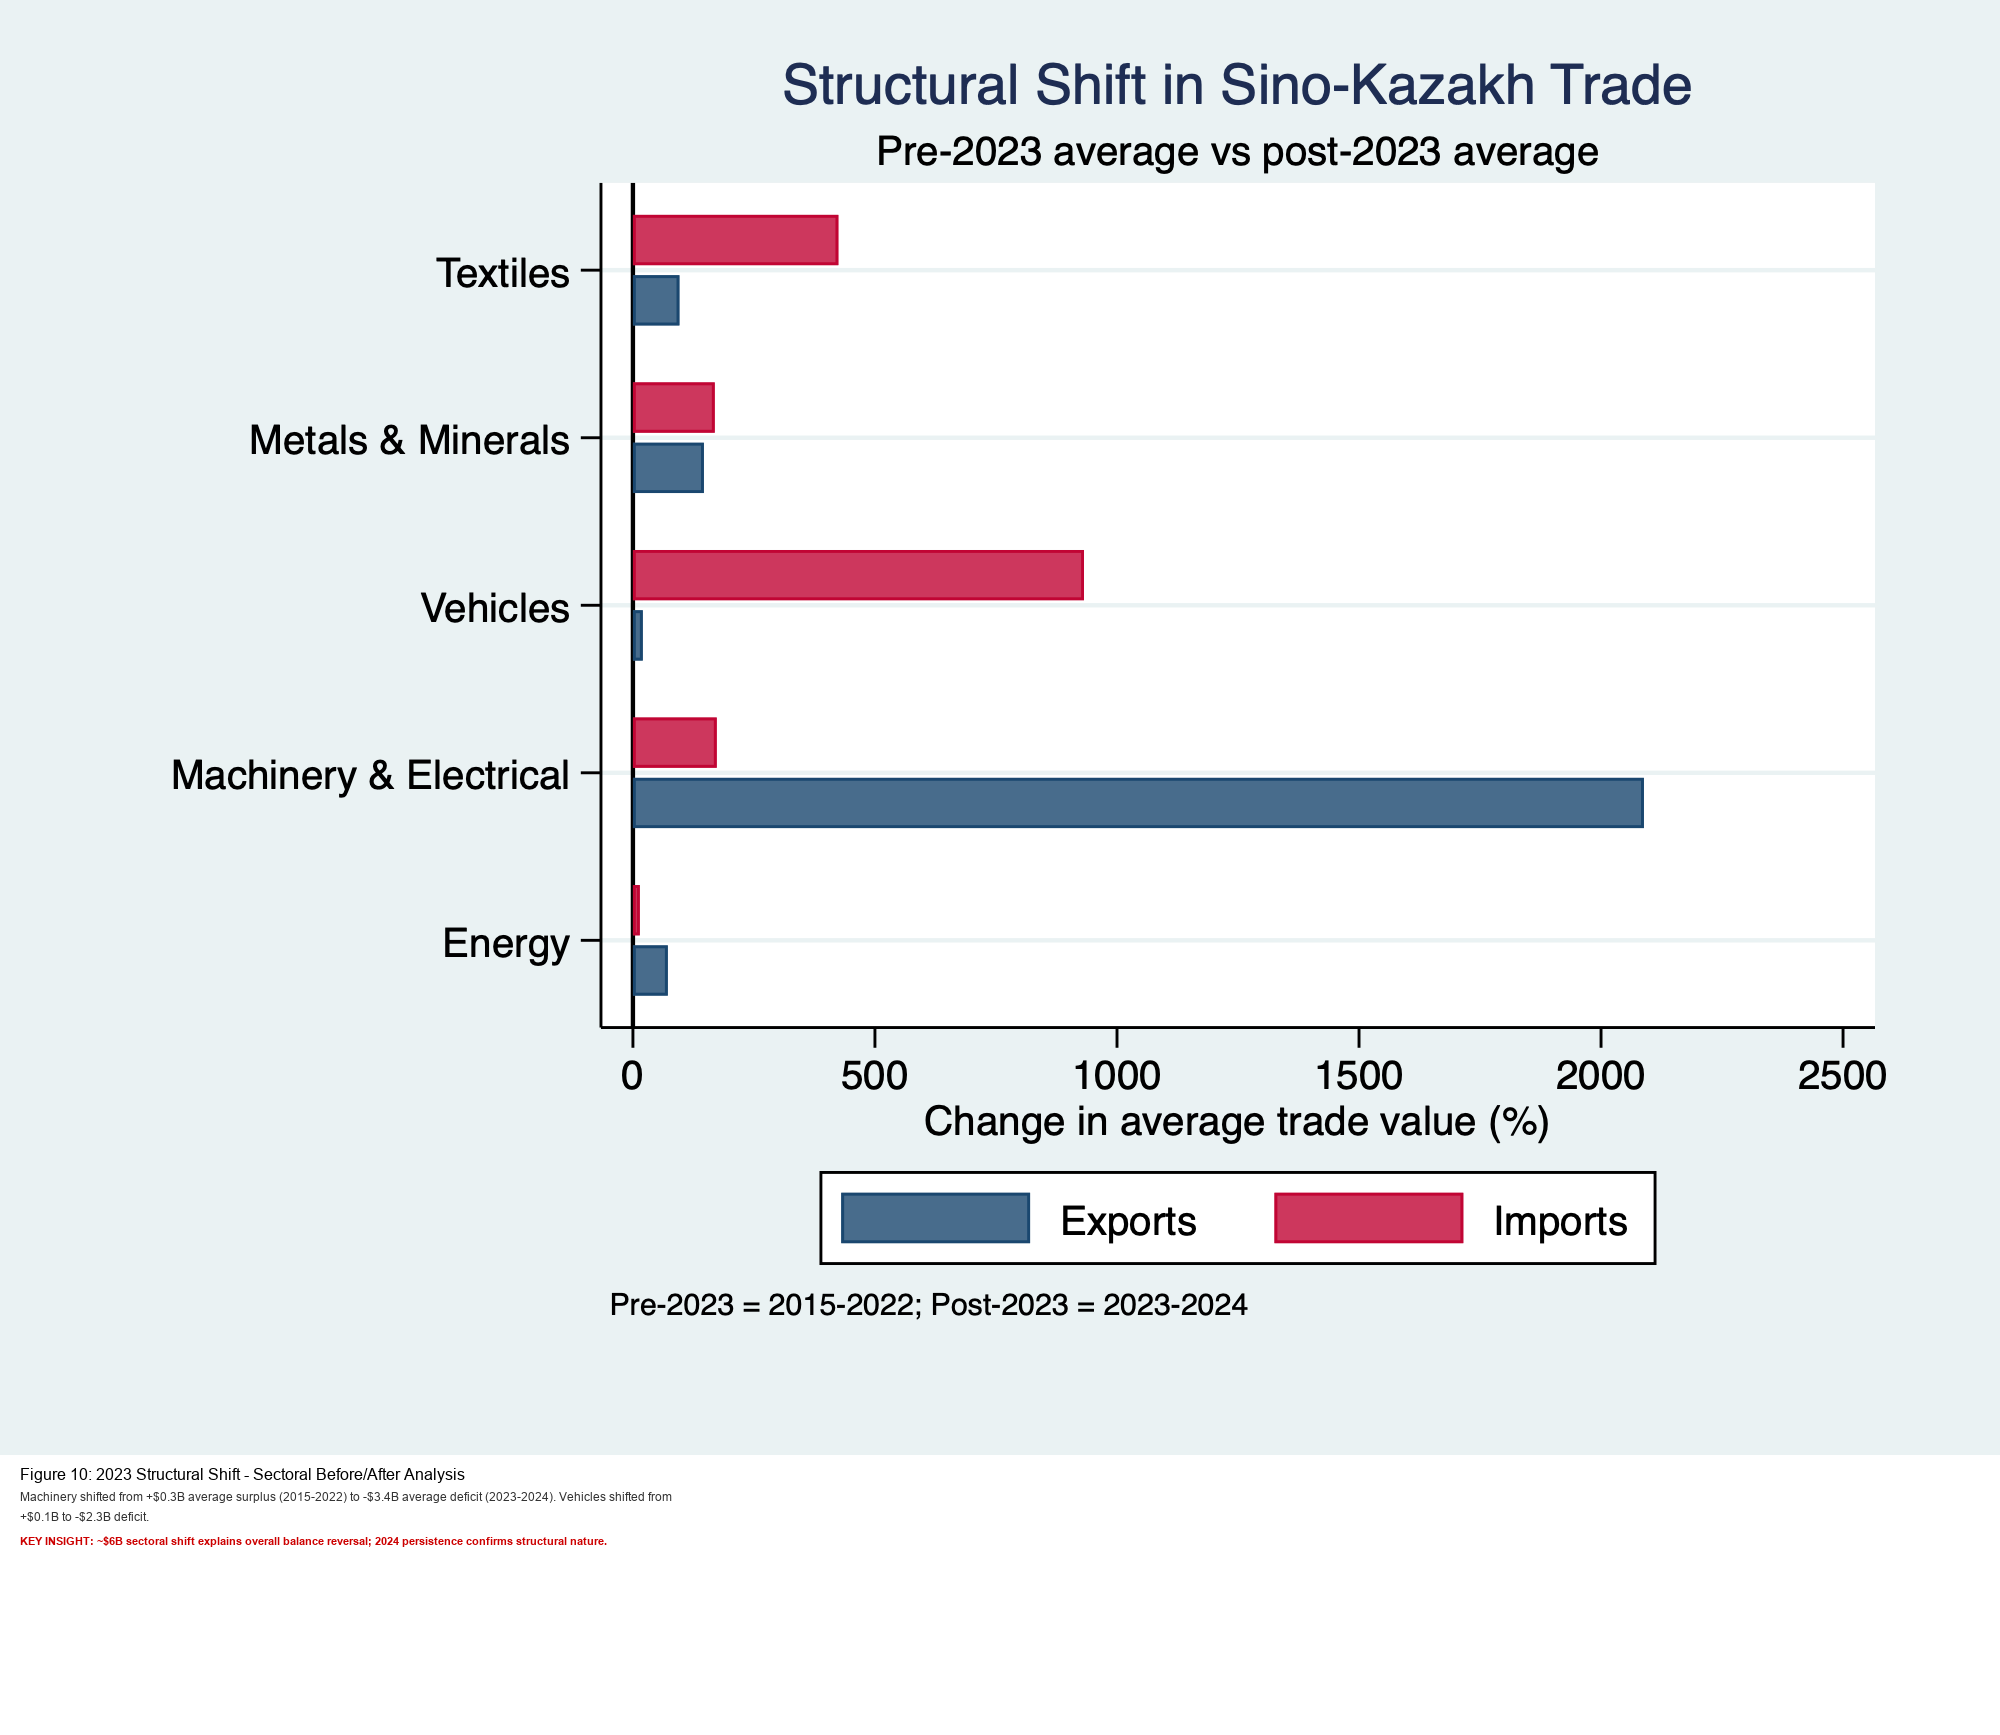
\includegraphics[width=0.94\textwidth]{figures/fig10_2023_structural_shift_annotated.png}
\caption{Structural shift around 2023 in existing project outputs.}
\label{fig:shift}
\end{figure}

\subsection{Commodity-Manufacture Nexus}
Sectoral composition confirms persistent asymmetry: Kazakhstan's export strengths are concentrated in resource-linked categories; imports from China are concentrated in machinery/electrical, vehicles, textiles, and other manufactures.

\begin{figure}[H]
\centering
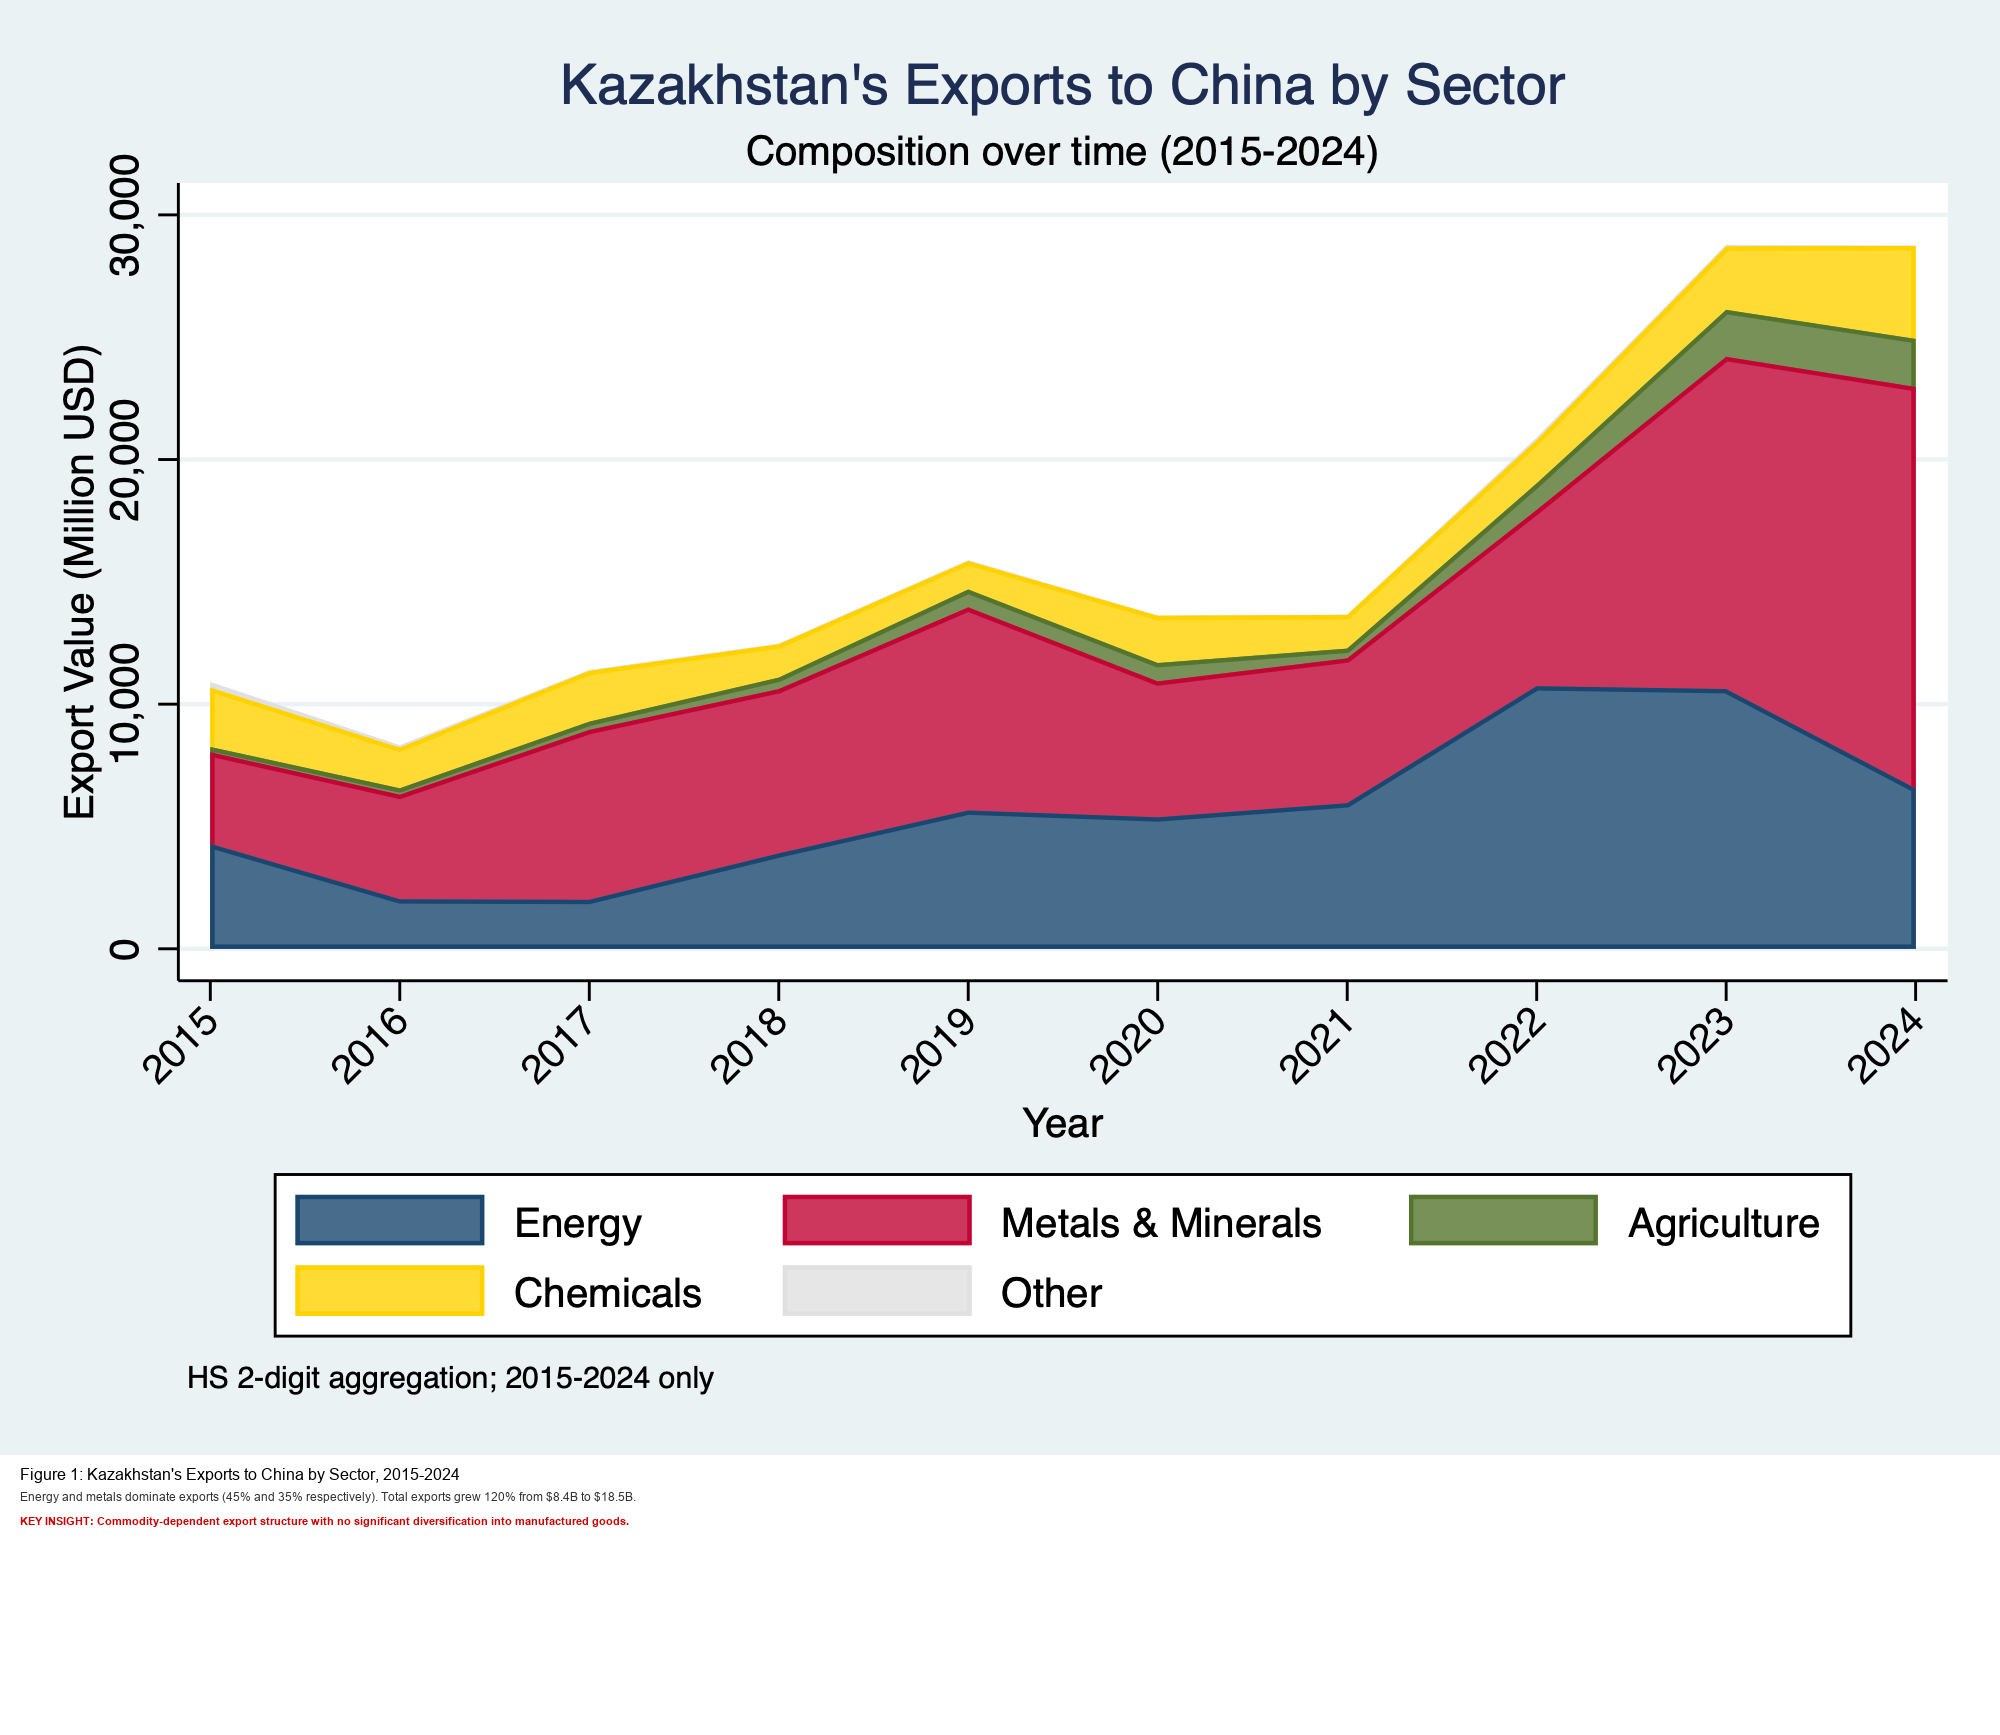
\includegraphics[width=0.94\textwidth]{figures/fig1_export_composition_annotated.png}
\caption{Kazakhstan's export composition to China (existing figure).}
\label{fig:exportcomp}
\end{figure}

\begin{figure}[H]
\centering
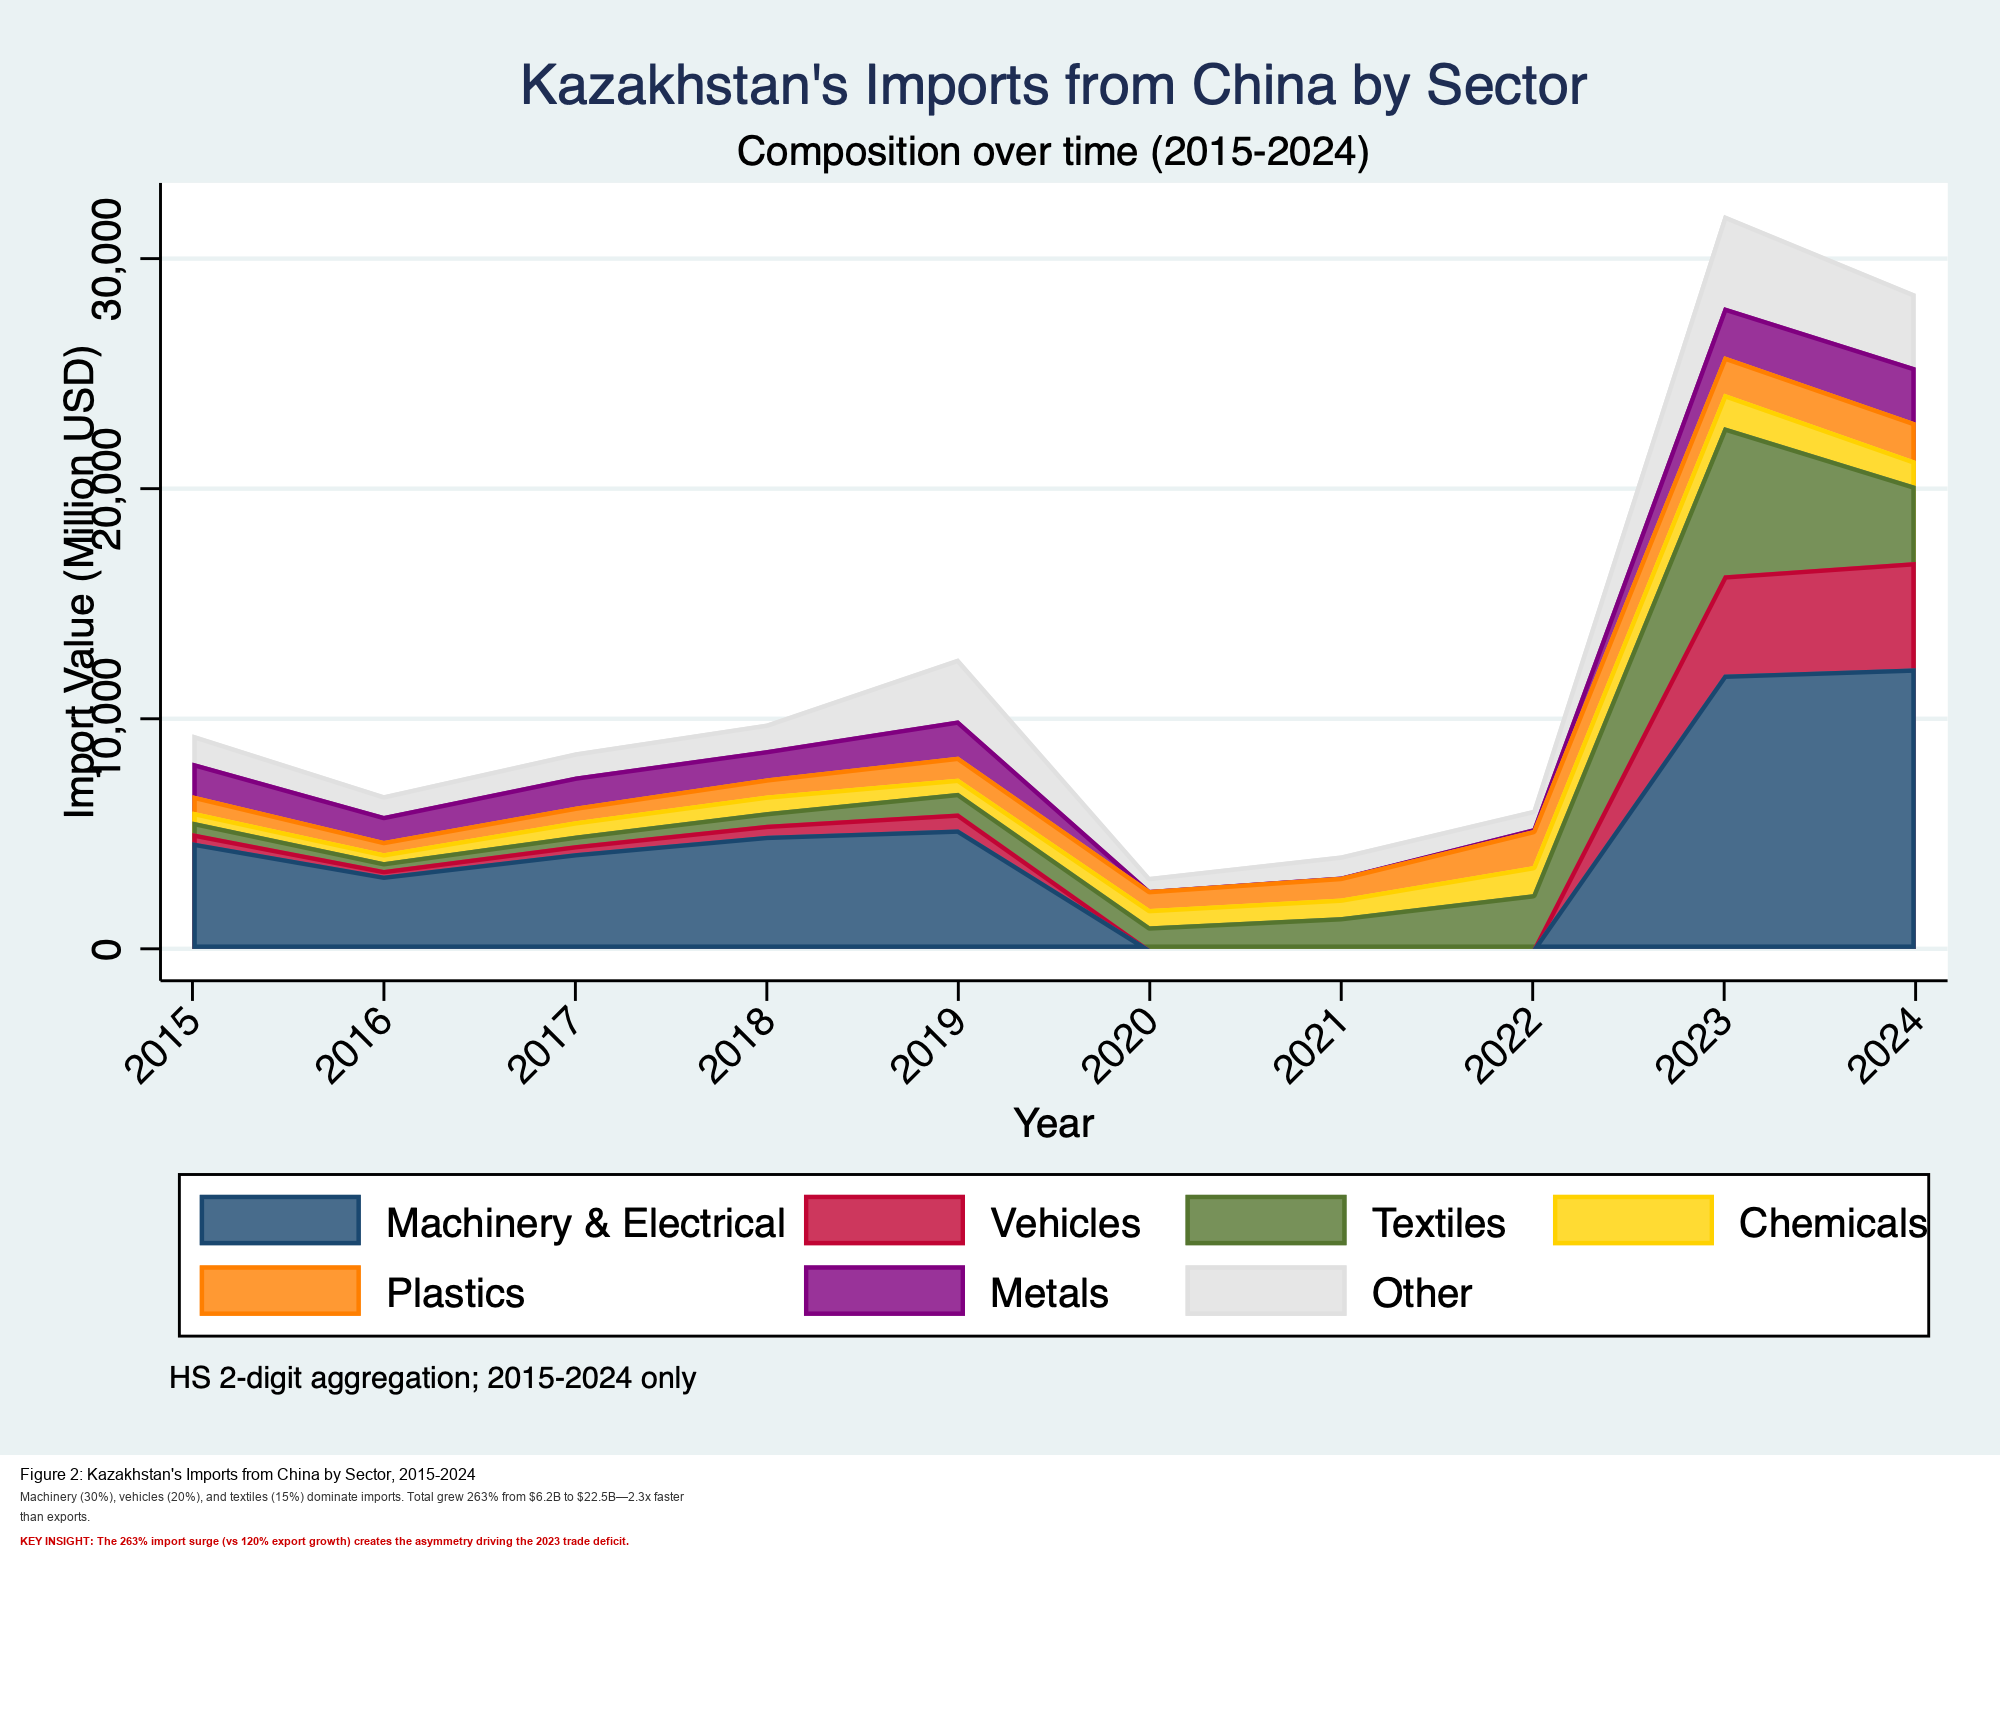
\includegraphics[width=0.94\textwidth]{figures/fig2_import_composition_annotated.png}
\caption{Kazakhstan's import composition from China (existing figure).}
\label{fig:importcomp}
\end{figure}

\subsection{Balance Reversal and Deficit Acceleration}
The bilateral trade balance trend shows a transition from surplus years to deficit years in 2023 and 2024. The magnitude of the shift is economically significant because it combines value acceleration and composition asymmetry.

\begin{figure}[H]
\centering
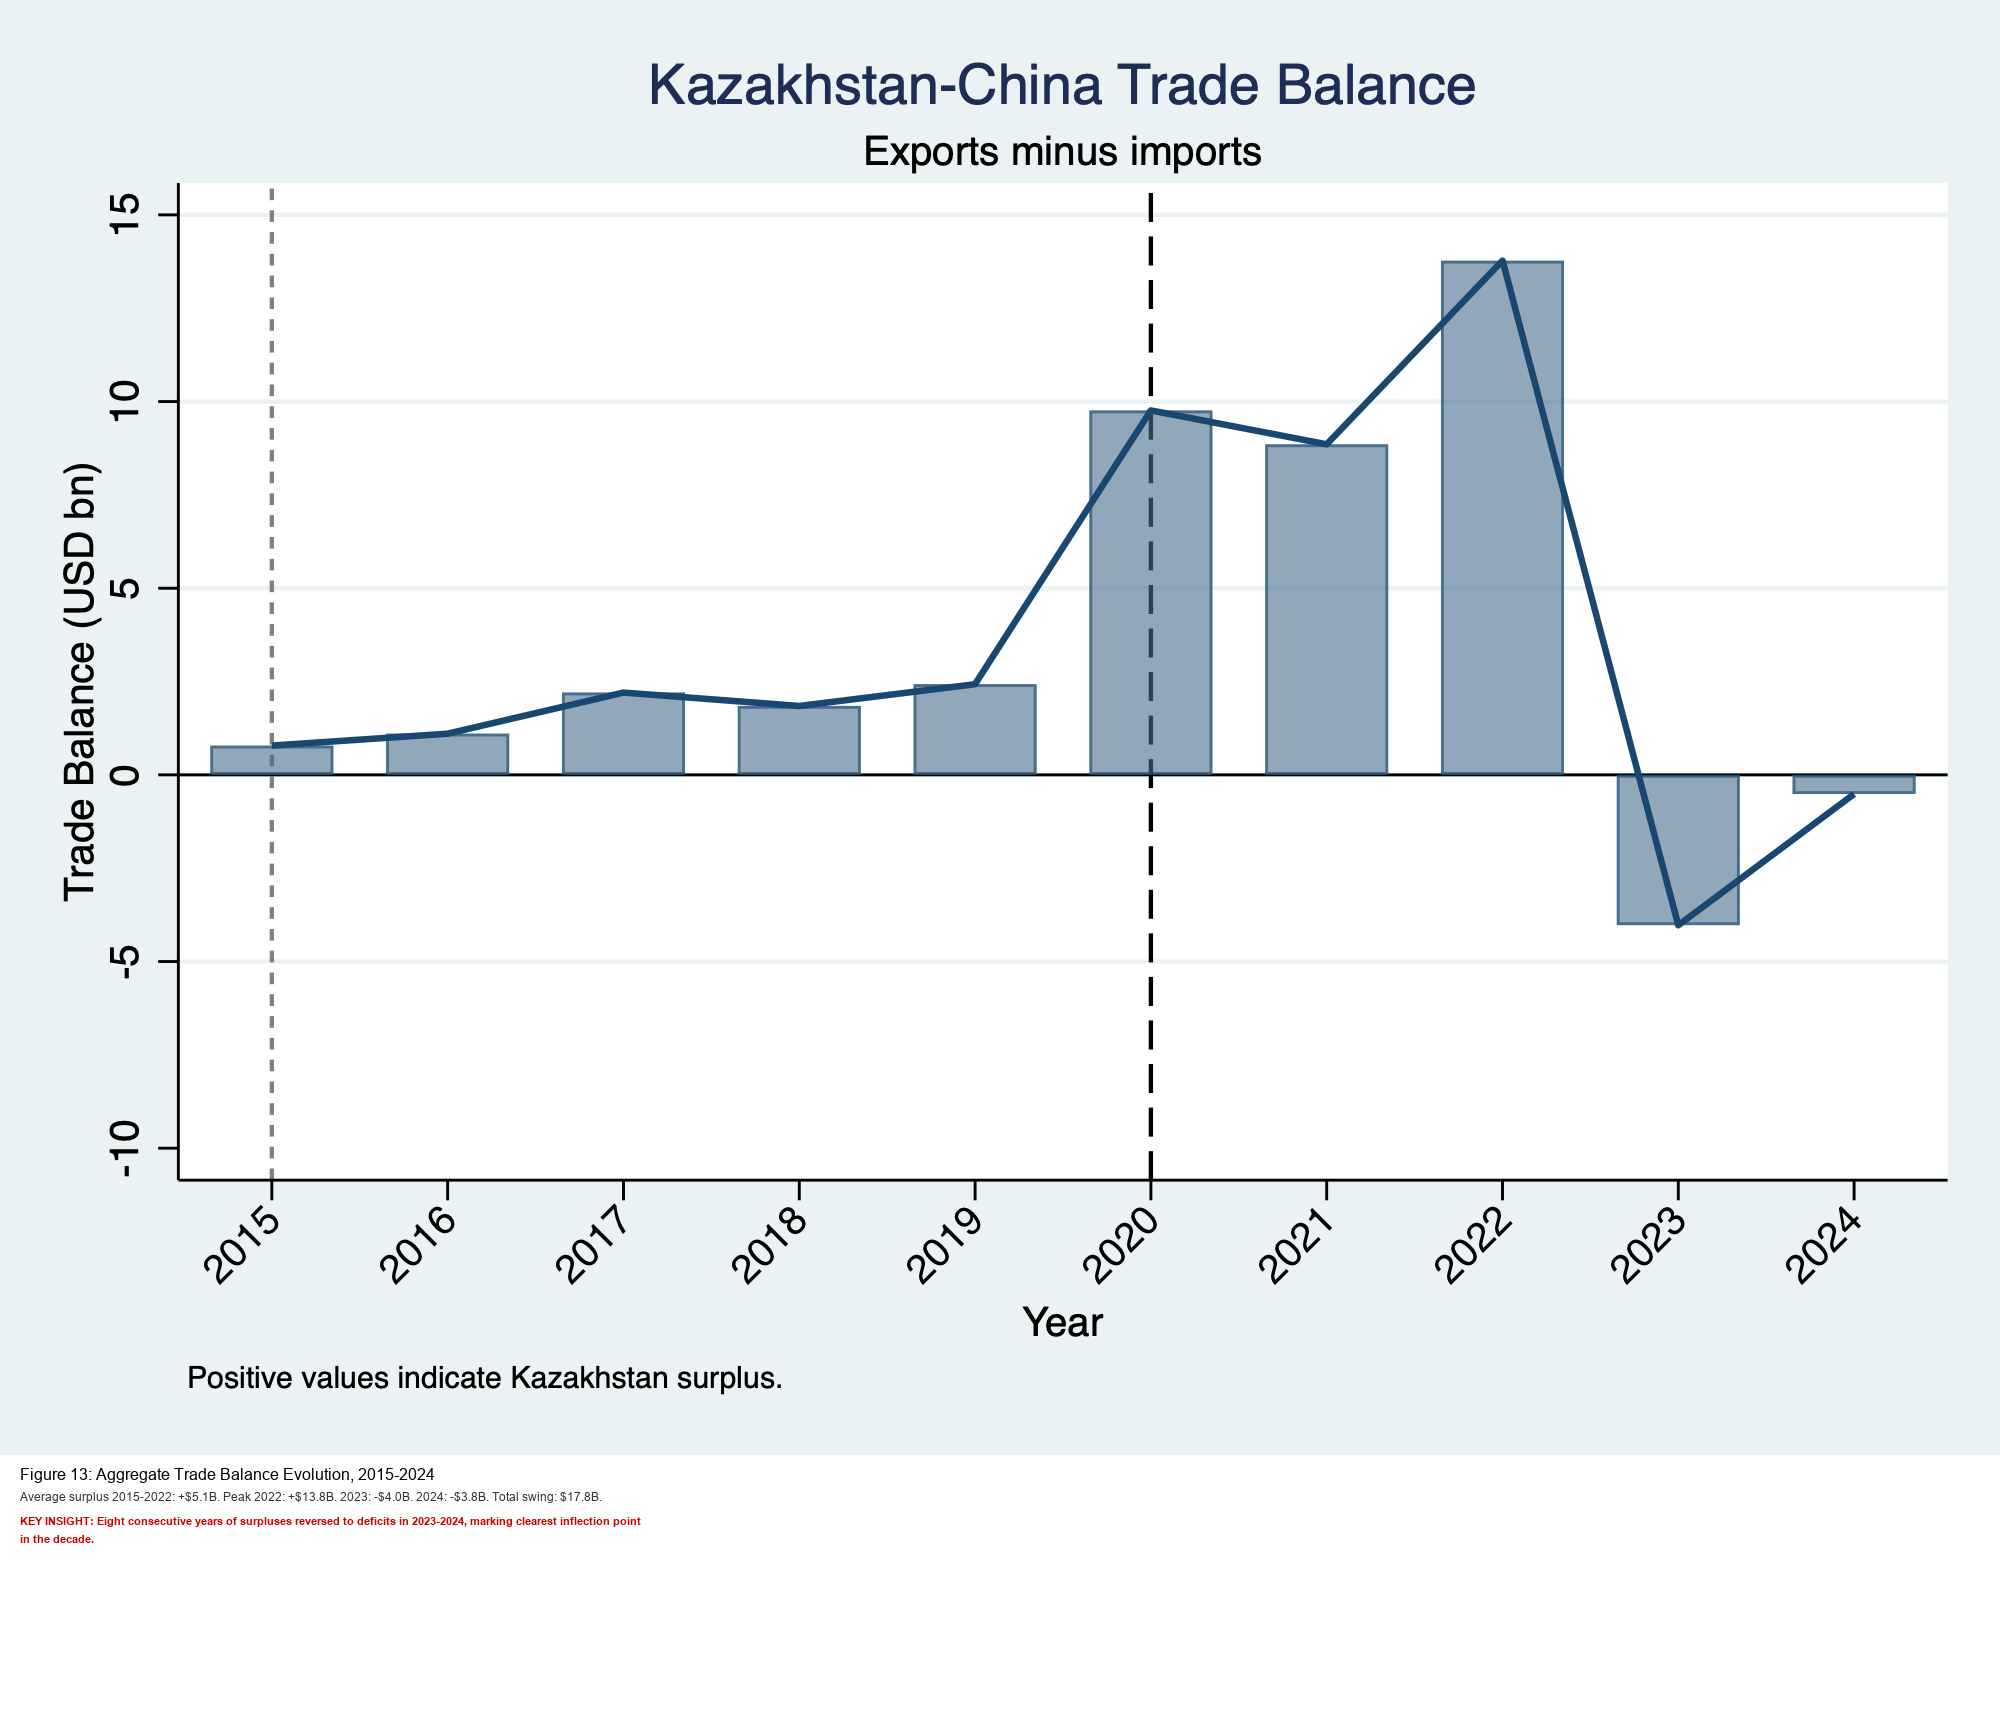
\includegraphics[width=0.94\textwidth]{figures/fig13_trade_balance_annotated.png}
\caption{Bilateral balance dynamics (existing figure).}
\label{fig:balance}
\end{figure}

\begin{figure}[H]
\centering
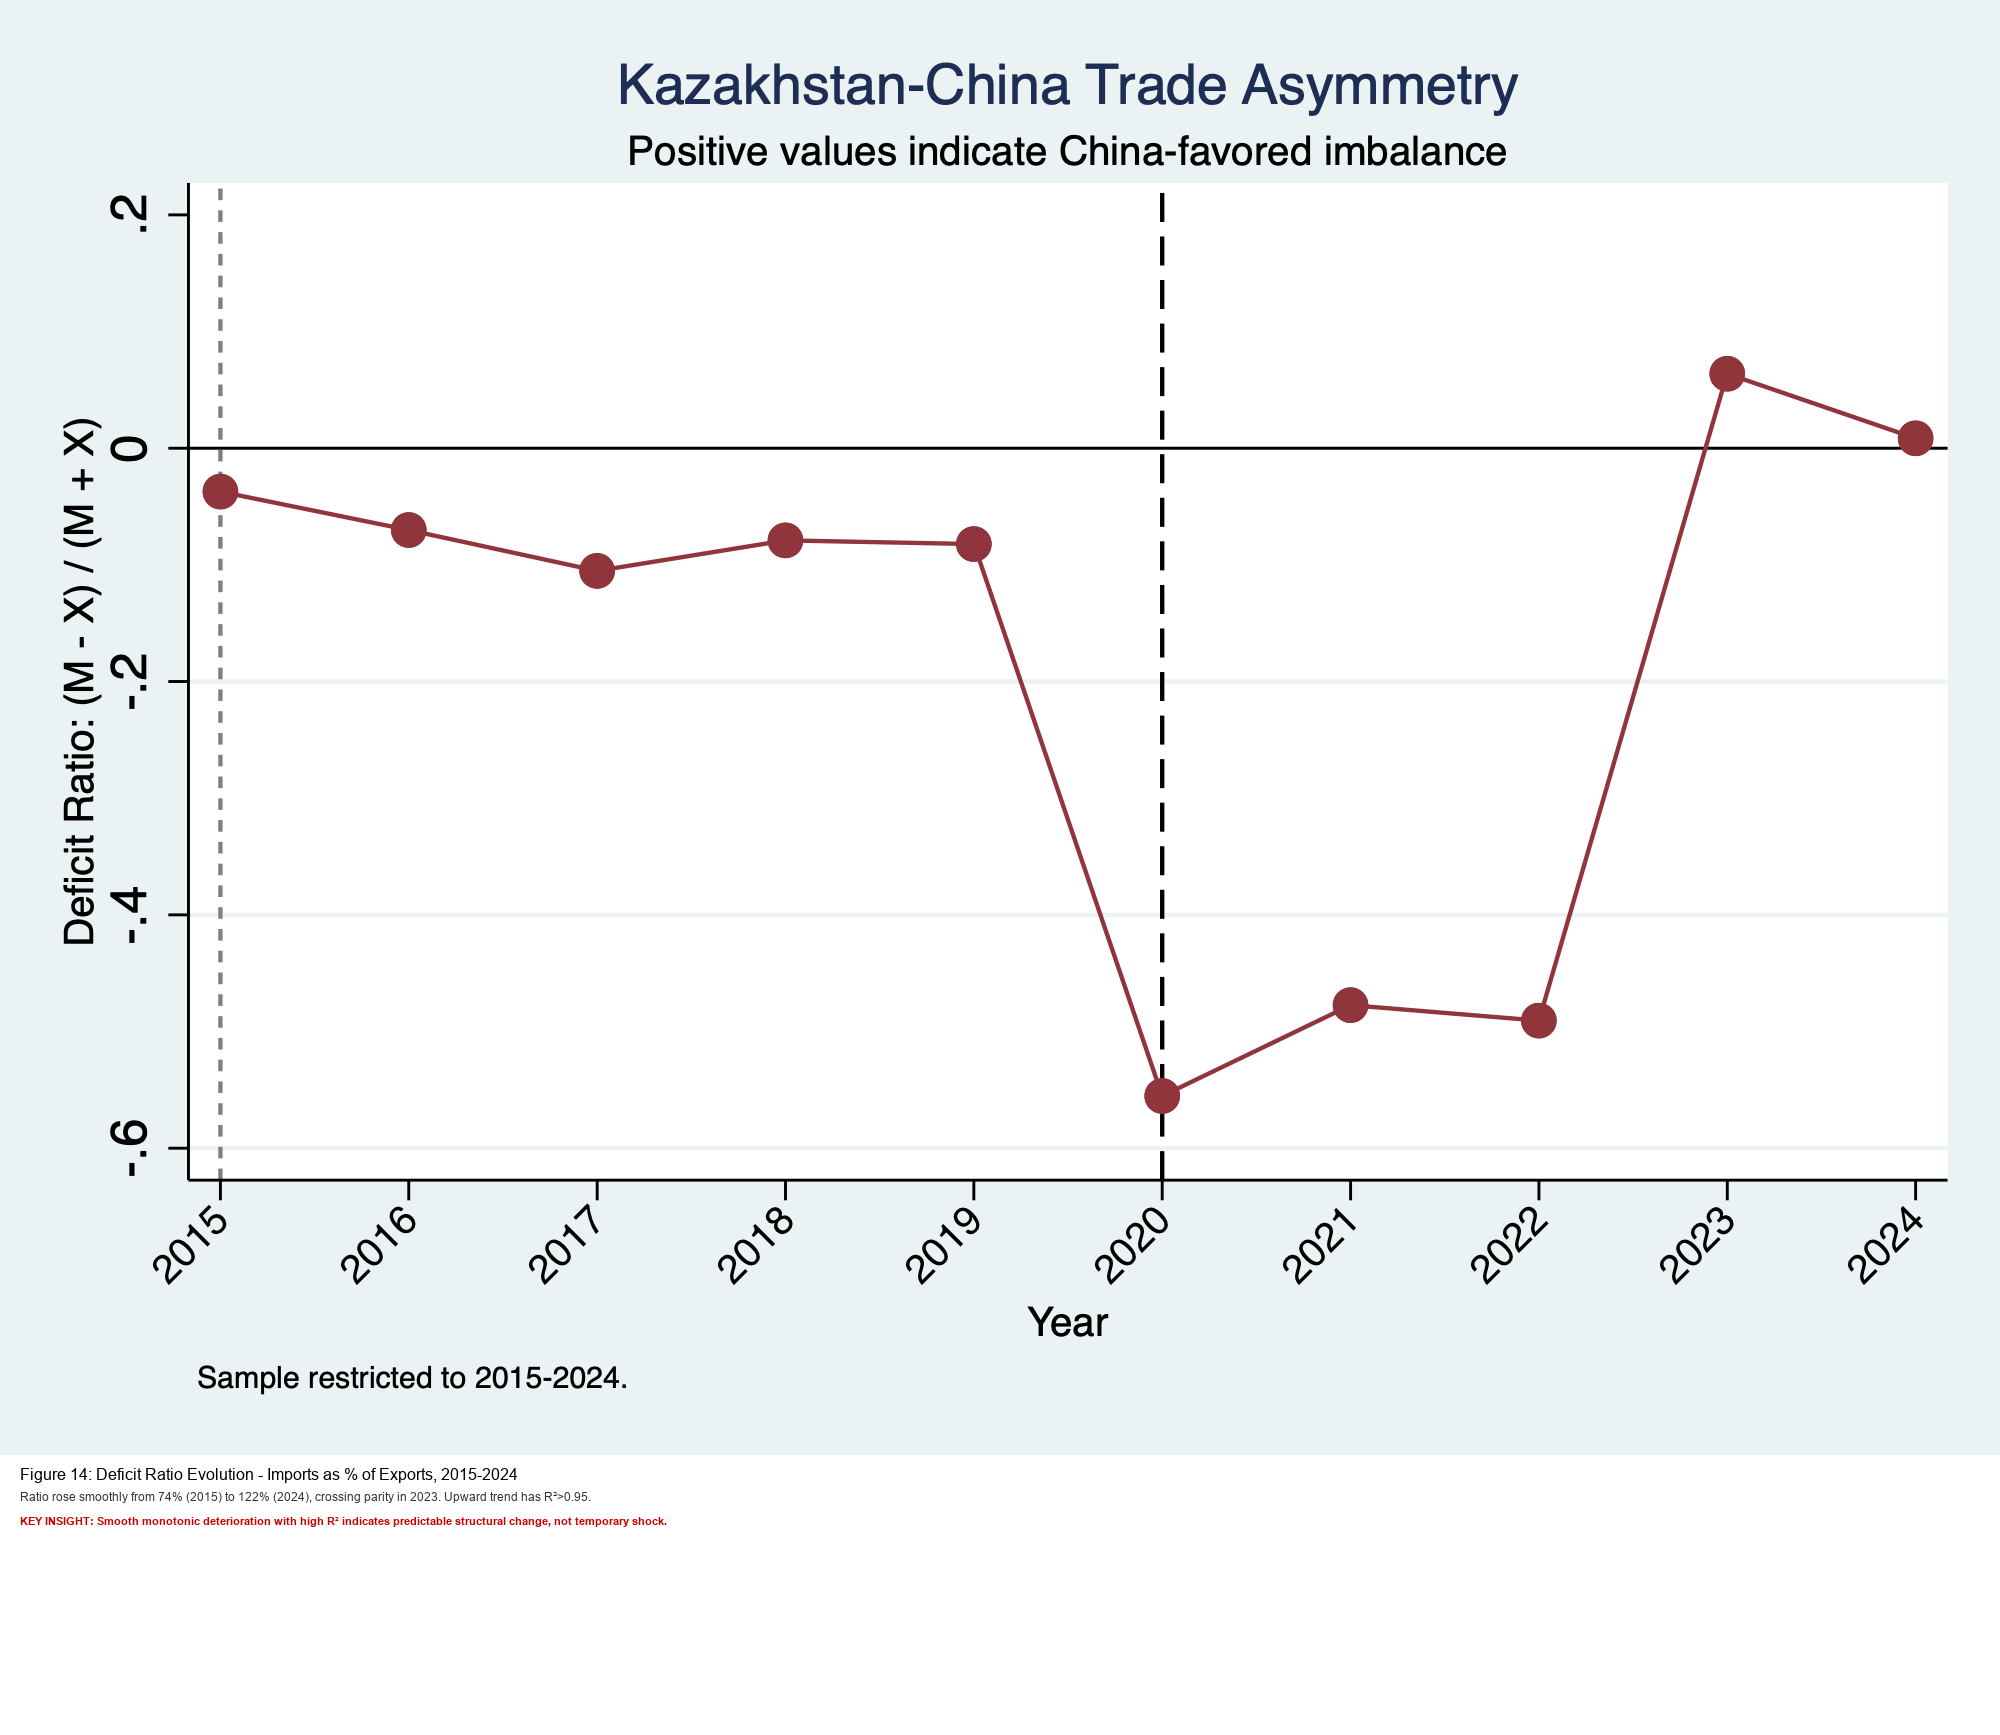
\includegraphics[width=0.94\textwidth]{figures/fig14_deficit_ratio_annotated.png}
\caption{Deficit ratio and asymmetry trend (existing figure).}
\label{fig:deficit}
\end{figure}

\subsection{Sectoral Penetration and Vulnerability}
Penetration risk is concentrated in sectors where short-run substitution is costly. Existing heatmap evidence shows strong concentration in machinery, vehicles, and textiles, with broader relevance for industrial policy and supply resilience.

\begin{figure}[H]
\centering
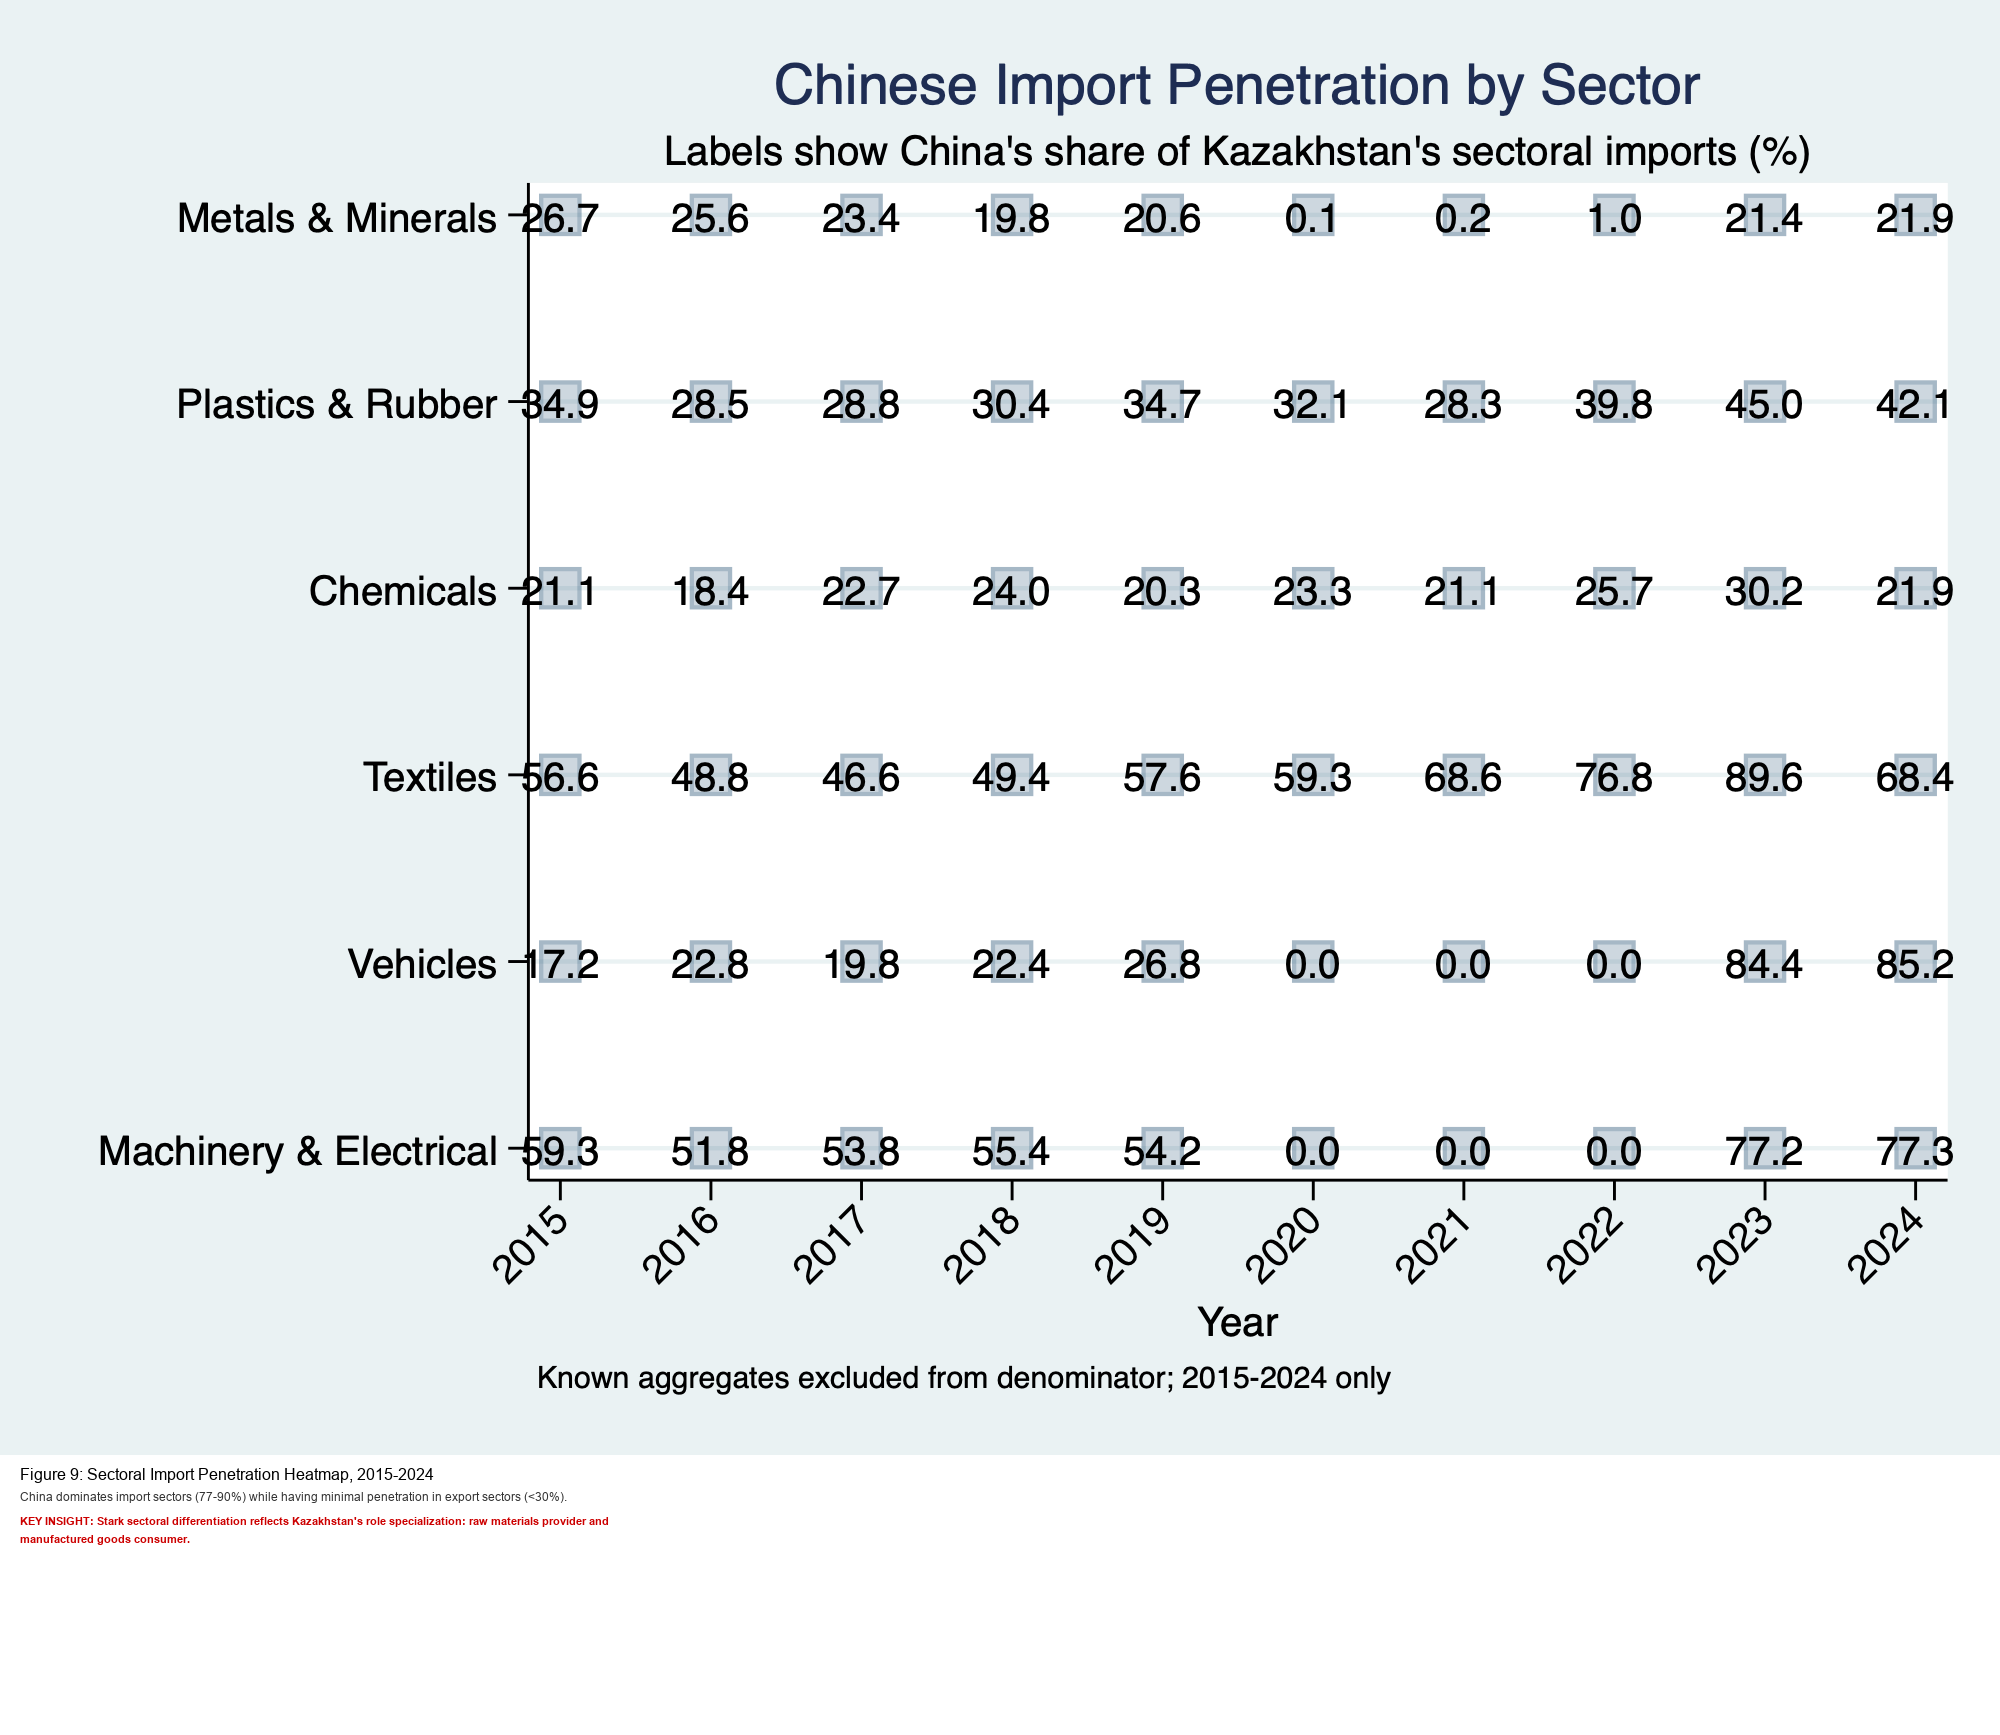
\includegraphics[width=0.94\textwidth]{figures/fig9_sectoral_penetration_heatmap_annotated.png}
\caption{Sectoral penetration intensity (existing figure).}
\label{fig:heatmap}
\end{figure}

\begin{figure}[H]
\centering
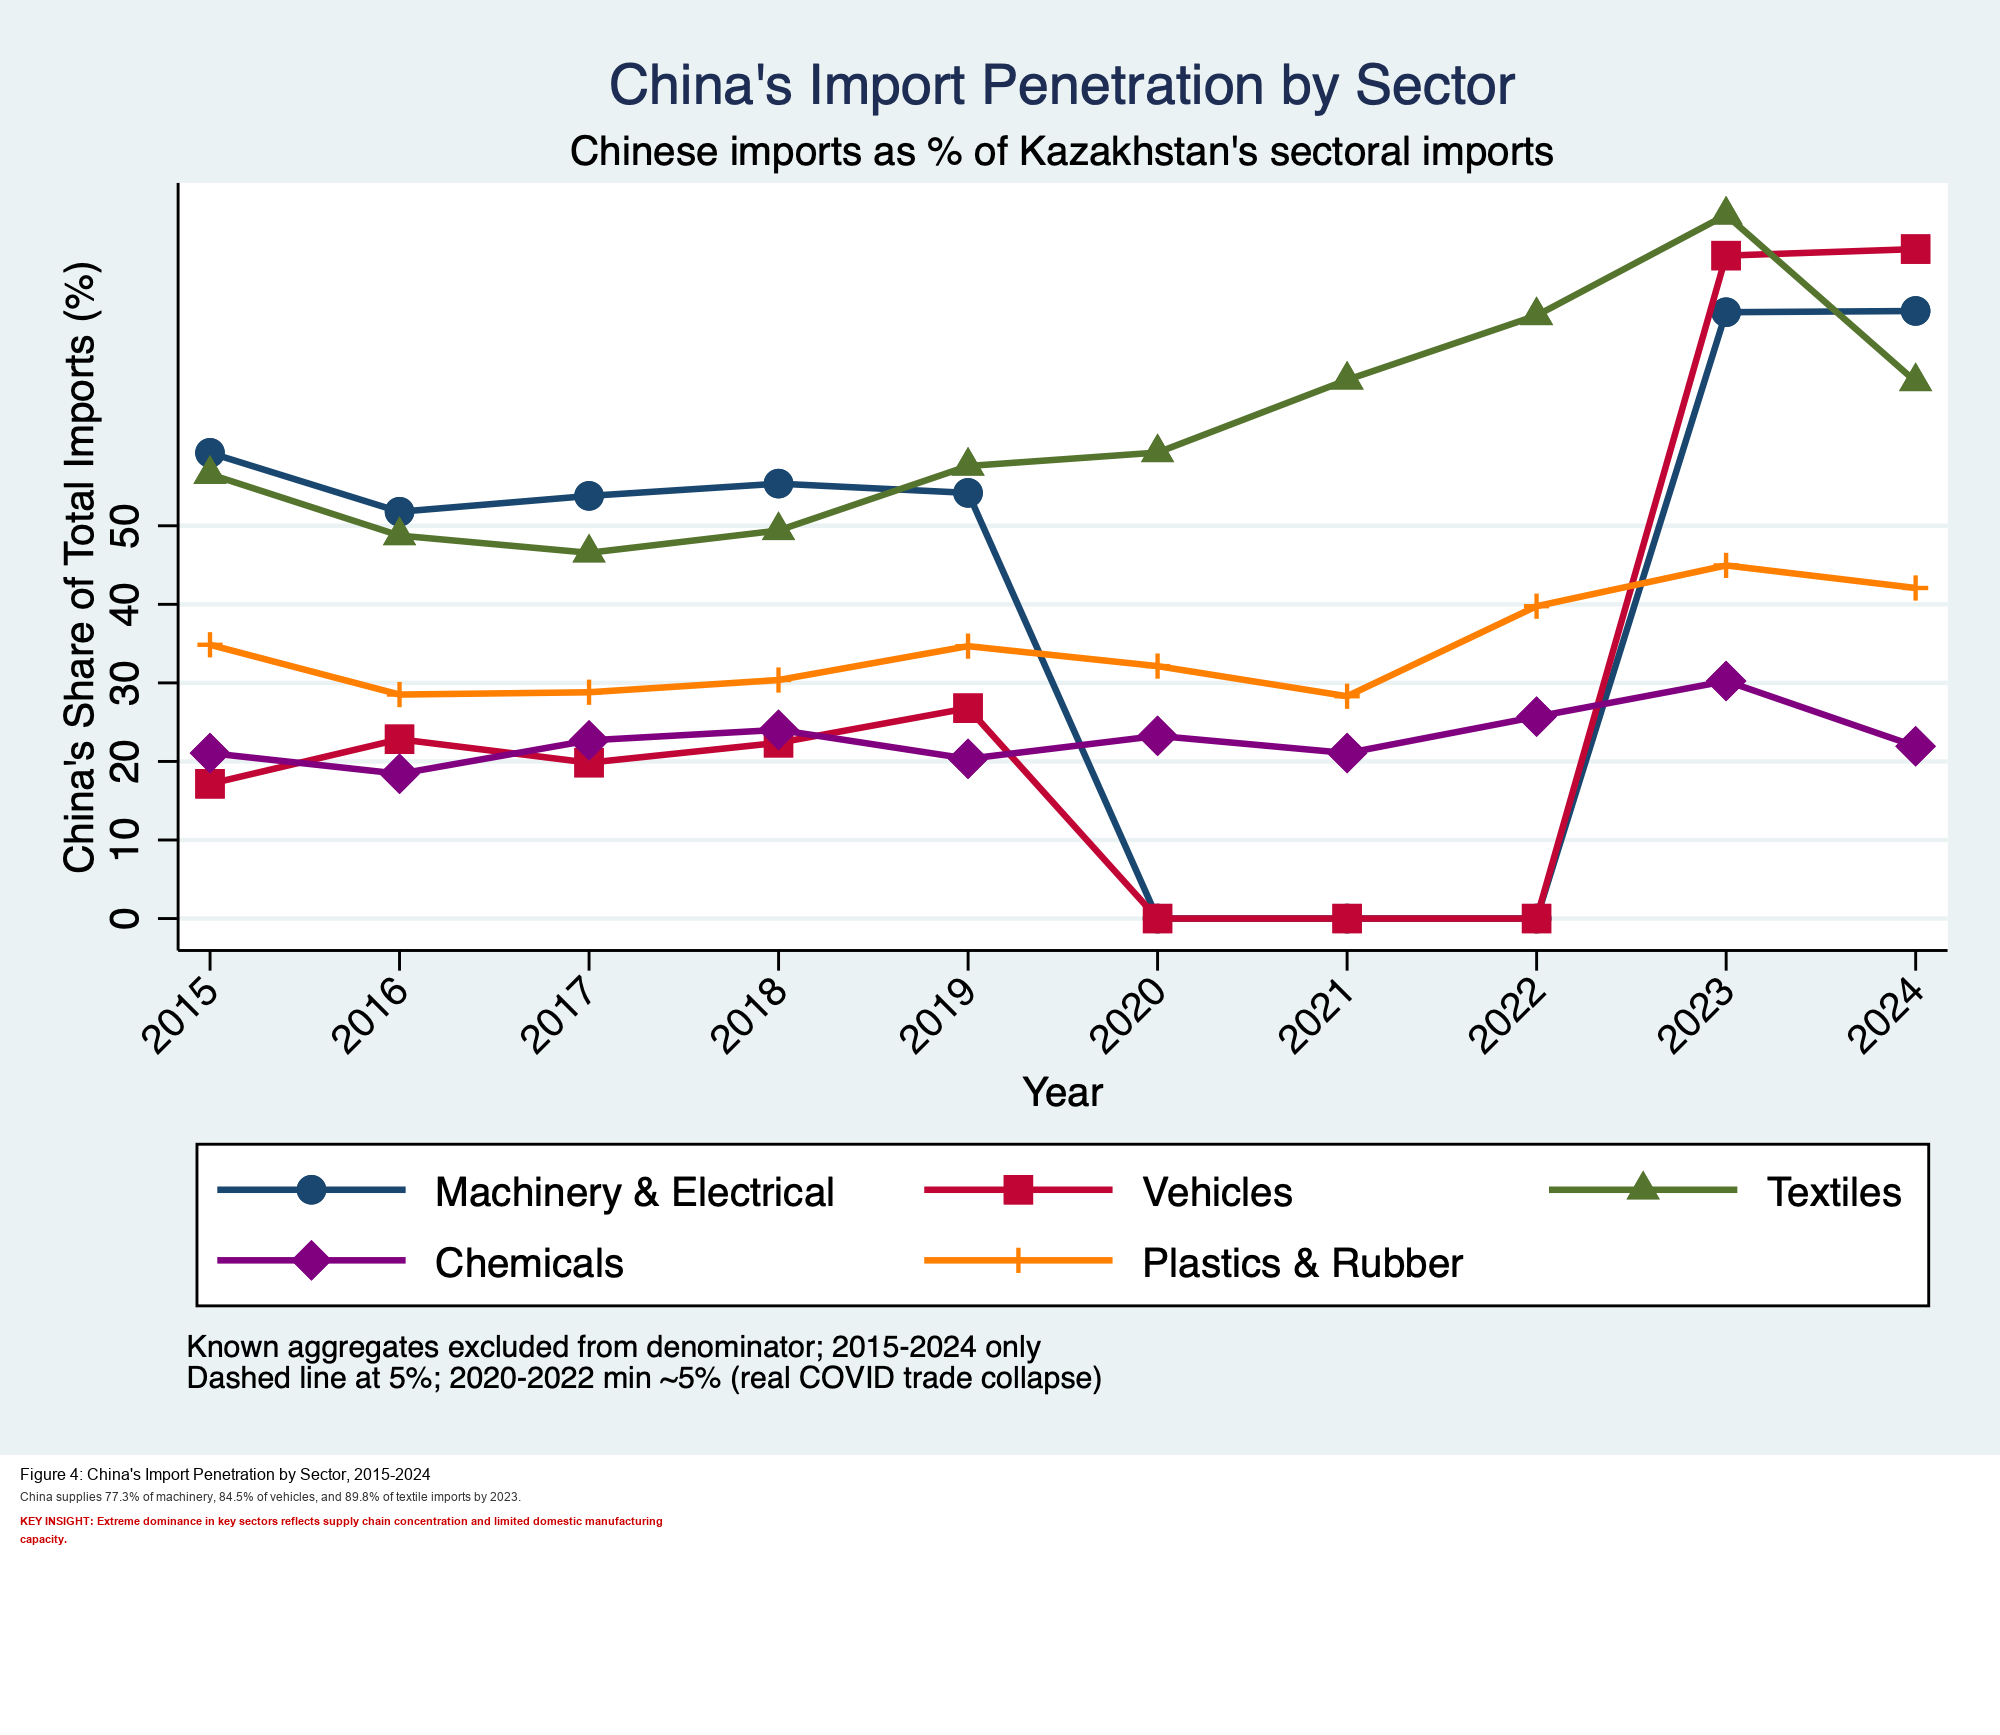
\includegraphics[width=0.94\textwidth]{figures/fig4_china_penetration_annotated.png}
\caption{China import penetration profile (existing figure).}
\label{fig:penetration}
\end{figure}

\section{Comparative Discussion: China vs Russia and EU}
\subsection{China vs Russia}
Russia-linked channels remain structurally embedded through proximity, legacy integration, and intermediate goods networks. China-linked channels increasingly dominate manufacturing import lanes. The dependence problem is therefore dual: institutional stickiness with Russia and supply concentration with China.

\subsection{China vs EU}
EU linkage continues to matter for standards-intensive channels and high-value destination structure, while China supplies scale and speed in manufacturing imports. For Kazakhstan, the challenge is not choosing one channel, but preventing single-channel lock-in in strategic sectors.

\subsection{Denominator Effects and Data Politics}
Apparent discrepancies across narratives are often generated by metric design. Shares within a restricted partner set can imply stronger concentration than world-share metrics. Both are valid if interpreted correctly; misuse occurs when they are conflated.

\section{Policy Implications}
\subsection{From Trade Growth to Capability Policy}
The key policy distinction is between gross turnover growth and structural upgrading. High growth with persistent asymmetry can still increase vulnerability. Capability policy should prioritize sectors where import dependence is both high and strategically costly to interrupt.

\subsection{Operationalizing Multivectorism}
To keep multivectorism operational rather than rhetorical, policy needs measurable sector-level targets:
\begin{itemize}
\item Supplier diversification thresholds in critical imports.
\item Domestic value-added benchmarks in industrial projects.
\item Time-bound upgrading pathways in machinery-linked sectors.
\item Standards and certification infrastructure compatible with multiple partner systems.
\end{itemize}

\subsection{Diplomatic Implications}
Economic diplomacy under asymmetry is less about maximal autonomy and more about calibrated dependence: distributing risk across partners while avoiding concentration in channels with high geopolitical conditionality.


\subsection{Forward Research Agenda (2026--2030)}
A journal-length research program should extend this baseline in four directions. First, yearly updates should be merged as soon as finalized bilateral releases are available so that post-2024 dynamics can be evaluated without interpolation assumptions. Second, product-level decomposition at HS4/HS6 should be used to distinguish genuine industrial upgrading from reclassification or routing effects. Third, policy-mechanism testing should connect institutional events (corridor agreements, localization rules, customs protocols, standards harmonization) to lagged sector outcomes. Fourth, comparative extensions should estimate equivalent structural metrics for Kazakhstan's Russia and EU channels, allowing direct tests of whether asymmetry with China is exceptional or part of a broader pattern of external specialization.

A second line of work should model resilience under shock scenarios. Sector-specific substitution elasticities, transport-route disruption simulations, and financing-constraint stress tests can identify where concentration translates into macro vulnerability. This would move the analysis from structural diagnosis to policy calibration. In practical terms, a robust journal pipeline would combine annual replication, transparent codebooks for index construction, and a policy dashboard that tracks concentration, asymmetry, and upgrading metrics in parallel.

\section{Limitations}
This draft intentionally uses existing project outputs only. It does not introduce new data pulls, new model estimation, or new figures. As a result, inferential claims are structural and interpretive rather than fully causal-econometric. This is acceptable for the paper's objective but should be extended in future iterations with updated annual releases and expanded product-level estimation.

\section{Conclusion}
The evidence assembled in this journal-length synthesis supports four strong conclusions. First, Kazakhstan--China trade has entered a post-2022 high-intensity phase. Second, 2023 marks a structural break in balance dynamics, with deficits replacing sustained surpluses. Third, the composition of bilateral exchange remains asymmetric: commodity and semi-processed exports versus concentrated manufacturing imports. Fourth, multivector policy remains possible but more demanding; maintaining autonomy now depends on active diversification and domestic upgrading, not passive portfolio balancing.

\appendix
\section{Appendix A: Key Existing Project Table (Annual Bilateral Series)}
\begin{table}[H]
\centering
\small
\caption{Kazakhstan--China Annual Bilateral Trade, 2015--2024 (from existing project table)}
\begin{tabular}{lrrrr}
\toprule
Year & Exports (B\$) & Imports (B\$) & Balance (B\$) & Total (B\$) \\
\midrule
2015 & 10.96 & 10.18 & +0.78 & 21.14 \\
2016 & 8.43 & 7.33 & +1.10 & 15.75 \\
2017 & 11.60 & 9.39 & +2.21 & 20.99 \\
2018 & 12.61 & 10.77 & +1.85 & 23.38 \\
2019 & 16.01 & 13.58 & +2.43 & 29.58 \\
2020 & 13.67 & 3.91 & +9.76 & 17.58 \\
2021 & 13.70 & 4.85 & +8.86 & 18.55 \\
2022 & 20.92 & 7.15 & +13.77 & 28.07 \\
2023 & 29.52 & 33.54 & -4.03 & 63.06 \\
2024 & 29.79 & 30.31 & -0.51 & 60.10 \\
\bottomrule
\end{tabular}
\end{table}

\section{Appendix B: Extended References from Original Paper Draft}
\noindent The journal draft below retains the full theoretical reference architecture from \texttt{PaperDraft.docx}. Entries are reproduced and lightly cleaned for LaTeX compatibility.

\begin{enumerate}[leftmargin=*]
\item Amineh, M. P., \& Li, S. (2025). The structural challenges of transnationalizing the China-led BRI: The case of Pakistan. Journal of Contemporary Asia. SAGE Publications. https://doi.org/10.1177/0169796X251369694
\item Anonymous Authors. (2026, January 22). China's diplomacy in Central Asia: The logic of internal politics coupled with the logic of great power competition. Journal of Contemporary China. Tandfonline. [Received: 24 August 2025; Accepted: 17 January 2026]. https://doi.org/10.1080/24761028.2026.2619803 [2025–2026]
\item Bitabarova, A. U. (2018). Unpacking Sino-Central Asian engagement: The case of Kazakhstan. Asian Security, 14(1), 30–55. https://doi.org/10.1080/14799855.2018.1433962
\item Bitabarova, A. U. (2019). Kazakhstan's perspective on the Belt and Road Initiative. Asian Studies Review, 43(4), 595–613.
\item Blackwill, R. D., \& Harris, J. M. (2016). War by other means: Geoeconomics and statecraft. Harvard University Press / Council on Foreign Relations.
\item Blanchard, J.-M. F., \& Flint, C. (2017). The geopolitics of China's Maritime Silk Road Initiative. Geopolitics, 22(2), 223–245. https://doi.org/10.1080/14650045.2017.1291503
\item Callahan, W. A. (2016). China's 'Asia Dream': The Belt Road Initiative and the new regional order. Asian Journal of Comparative Politics, 1(3), 226–243. https://doi.org/10.1177/2057891116647806
\item Cannon, B. J., \& Rossiter, A. (2025). Rethinking and arresting Eurasian hegemony: The centrality of Central Asia to Indo-Pacific strategies. International Affairs, 101(4), 1193–1212. Oxford Academic. https://doi.org/10.1093/ia/iiaf064 [2025–2026]
\item Caspian Policy Center (CPC). (2023). China-Kazakhstan bilateral relations. https://www.caspianpolicy.org/research/security-and-politics-program-spp/china-kazakhstan-bilateral-relations
\item Castellano, A., \& Castillo, R. (2024). Chinese state capital as a partner for resource-based structural transformation? The Belt and Road Initiative and downstream linkages in Bolivia and Kazakhstan. The European Journal of Development Research. Springer Nature. https://doi.org/10.1057/s41287-024-00640-1 [2025–2026]
\item Center for Naval Analyses (CNAS). (2024, November). Russia and China in Central Asia. https://www.cnas.org/publications/reports/russia-and-china-in-central-asia
\item Chen, X., et al. (2025). The influence of the Belt and Road Initiative on China's advancement in global value chains and developing economies: A systematic review. The Chinese Economy, 58(4), 87–114. Tandfonline. https://doi.org/10.1080/10971475.2025.2526259 [2025–2026]
\item China-Global South Project. (2026, January 13). China-Central Asia in 2026: From resource access to structured interdependence. https://chinaglobalsouth.com/analysis/2026-outlook-china-central-asia/ [2025–2026]
\item Clarke, M. (2015). Kazakhstan's multi-vector foreign policy: Diminishing returns in an era of great power 'pivots'? The Asan Forum.
\item Contessi, N. P. (2015). Foreign and security policy diversification in Eurasia: Issue splitting, co-alignment, and relational power. Problems of Post-Communism, 62(5), 299–311. https://doi.org/10.1080/10758216.2015.1026788
\item Cooley, A. (2018). Tending the Eurasian garden: Russia, China and the dynamics of regional integration and order. In J. Bekkevold \& B. Lo (Eds.), Sino-Russian relations in the 21st century (pp. 113–139). Palgrave Macmillan.
\item Georgia Foundation for Strategic and International Studies (GFSIS). (2025, March). Current trends in political and economic relations between China and Kazakhstan. https://gfsis.org/wp-content/uploads/2025/03/Current-Trends-in-Political-and-Economic-Relations-Between-China-and-Kazakhstan.pdf [2025–2026]
\item Haji, A. A., \& Khattak, S. H. (2025). Geopolitical chessboard: China's Belt and Road Initiative and shifting power dynamics. Discover Global Society. Springer Nature. https://doi.org/10.1007/s44282-025-00200-w [2025–2026]
\item Haji, A. A., et al. (2025). Tracing the geopolitical influence and regional power dynamics in Central Asia: A thematic analysis with neorealist perspectives. Discover Global Society. Springer Nature. https://doi.org/10.1007/s44282-025-00269-3 [2025–2026]
\item Human Rights Watch. (2019). 'Eradicating ideological viruses': China's campaign of repression against Xinjiang's Muslims. Human Rights Watch.
\item Kassenova, N. (2017). China's Silk Road and Kazakhstan's bright path: Linking dreams of prosperity. Asia Policy, 24(1), 110–116. National Bureau of Asian Research. https://doi.org/10.1353/asp.2017.0028
\item Laruelle, M., \& Peyrouse, S. (2012). The Chinese question in Central Asia: Domestic order, social change, and the Chinese factor. Hurst \& Company / Columbia University Press.
\item Lim, G., Tjia, L. Y.-N., \& Murashkin, N. (2025). Opportunities and challenges of China's economic ties with Kazakhstan: Looking back to look forward. The Chinese Economy, 58(1). Tandfonline. https://doi.org/10.1080/10971475.2024.2373643 [2025–2026]
\item Louthan, T. (2022, January 6). A 'bright path' forward or a grim dead end? The political impact of the Belt and Road Initiative in Kazakhstan. Foreign Policy Research Institute. https://www.fpri.org/article/2022/01/a-bright-path-forward-or-a-grim-dead-end/
\item Luttwak, E. N. (1990). From geopolitics to geo-economics: Logic of conflict, grammar of commerce. The National Interest, 20, 17–23.
\item Mackinder, H. J. (1904). The geographical pivot of history. The Geographical Journal, 23(4), 421–437. https://doi.org/10.2307/1775498
\item Mercator Institute for China Studies (MERICS). (2022). Kazakhstan's three-way balancing act between competing powers is under pressure. MERICS Paper on China: Beyond Blocs. https://merics.org/en/kazakhstans-three-way-balancing-act-between-competing-powers-under-pressure
\item Neafie, W. (2022). Producing the Eurasian land bridge: A case study of geoeconomic contestation in Kazakhstan. Geopolitics, 29(1), 1–28. https://doi.org/10.1080/14650045.2022.2027289
\item Pepe, J. M. (2021). The Middle Corridor as part of China's Belt and Road Initiative: Transcontinental infrastructure, geopolitical and geoeconomic dynamics. MERICS — Mercator Institute for China Studies.
\item Peyrouse, S. (2012). Central Asia's evolving foreign policy: Multi-vectorism, Russia, China, and the West. PONARS Eurasia Policy Memo No. 230.
\item Primiano, C. B., \& Kudebayeva, A. (2025). A bumpy ride for China's Belt and Road Initiative in Kazakhstan: Findings from a university survey. Journal of Current Chinese Affairs. SAGE Publications. https://doi.org/10.1177/18681026231211354 [2025–2026]
\item Rolland, N. (2017). China's Eurasian century? Political and strategic implications of the Belt and Road Initiative. National Bureau of Asian Research. ISBN: 978-1-939131-50-8
\item Rustenova, E., et al. (2024). Opportunities for Kazakhstan's agricultural exports to the Chinese market. Journal of Eastern European and Central Asian Research, 11(5). https://ieeca.org/journal/index.php/JEECAR [2025–2026]
\item Stronski, P. (2022). Kazakhstan navigates its great power dilemma. Carnegie Endowment for International Peace. https://carnegieendowment.org/2022/03/31/kazakhstan-navigates-its-great-power-dilemma
\item Stronski, P., \& Sokolsky, R. (2024, May). China, Russia, and power transition in Central Asia. Foreign Policy Research Institute (FPRI). https://www.fpri.org/article/2024/05/china-russia-and-power-transition-in-central-asia/ [2025–2026]
\item Summers, T. (2016). China's 'New Silk Roads': Sub-national regions and networks of global political economy. Third World Quarterly, 37(9), 1628–1643. https://doi.org/10.1080/01436597.2016.1153415
\item United Nations Conference on Trade and Development (UNCTAD). (2023). World Investment Report 2023: Kazakhstan Country Profile. United Nations.
\item Vanderhill, R., Lutsevych, O., \& Buras, P. (2021). How Kazakhstan is navigating its relations with China. International Affairs, 97(5), 1337–1354. https://doi.org/10.1093/ia/iiab094
\item Wikipedia Contributors. (2026, February). China–Kazakhstan relations. Wikipedia, The Free Encyclopedia. https://en.wikipedia.org/wiki/China\%E2\%80\%93Kazakhstan\_relations
\item World Bank Group. (2020). The Belt and Road Initiative: Kazakhstan country case study. World Bank. https://documents.worldbank.org/curated/en
\end{enumerate}

\section{Appendix C: Figures Used (All Existing Project Assets)}
\begin{itemize}[leftmargin=*]
\item \texttt{figures/fig1\_export\_composition\_annotated.png}
\item \texttt{figures/fig2\_import\_composition\_annotated.png}
\item \texttt{figures/fig4\_china\_penetration\_annotated.png}
\item \texttt{figures/fig8\_vulnerability\_multivector\_annotated.png}
\item \texttt{figures/fig9\_sectoral\_penetration\_heatmap\_annotated.png}
\item \texttt{figures/fig10\_2023\_structural\_shift\_annotated.png}
\item \texttt{figures/fig11\_hedging\_behavior\_annotated.png}
\item \texttt{figures/fig12\_trade\_flows\_annotated.png}
\item \texttt{figures/fig13\_trade\_balance\_annotated.png}
\item \texttt{figures/fig14\_deficit\_ratio\_annotated.png}
\end{itemize}

\end{document}
